\subsection{Background information}
\label{sec:gbb-unfoldingintro}

The goal of unfolding\footnote{The text in this section is taken verbatim from Ref.~\cite{ATL-COM-PHYS-2014-767}.} is to correct the measured data for effects arising from the finite efficiency, acceptance and  
resolution of the detector. In this analysis an iterative Bayes unfolding technique was chosen to correct the data, the details of which will be given in what 
follows.

By treating each bin of a histogram as an element in a vector or matrix, we can write
\begin{equation}
  \mathbf{A\cdot x} = \mathbf{y}
  \label{eqn:unfolding:matrix}
\end{equation}
where $\mathbf{x}$ is the true distribution we are interested in, $\mathbf{y}$ is the distribution we
measure and $\mathbf{A}$ is a matrix -- often the "response", "smearing" or "transfer" matrix -- which encodes information
about the detector and transforms the distributions from true to measured.

After writing the problem as in equation~(\ref{eqn:unfolding:matrix}),
it is tempting to think that the solution is simply to
invert the matrix $\mathbf{A}$ and apply it to our measured distribution $\mathbf{y}$. However,
it is argued by D'Agostini~\cite{D'Agostini:1994zf} that since the problem of unfolding is inherently a probabilistic one, we should use probabilistic methods to solve
it.

The problem can be reformulated by writing the \emph{probability} for finding an event in bin $i$ of the true distribution, $d^\prime_i$, as
\begin{equation}
  d^\prime_i = \sum_j\mathrm{P}(T_i|M_j)\;d_j  = \sum_{j}\theta_{ij}\;d_j
  \label{eqn:unfolding:unfoldingmatrix}
\end{equation}
where $\mathrm{P}(T_i|M_j)$ is an element of the `unfolding matrix' $\theta_{ij}$ and gives us the probability for finding
an event in bin $i$ of the true distribution, given that we measured one in bin $j$. $d_j$ is the probability for finding
an event in bin $j$ of the measured distribution.

Using Bayes' theorem it is possible to rewrite the unfolding matrix as
\begin{equation}
  \theta_{ij} = \mathrm{P}(T_i|M_j) = \frac{\mathrm{P}(M_j|T_i)\cdot \mathrm{P}(T_i)}{\sum_i \mathrm{P}(M_j|T_i)\cdot \mathrm{P}(T_i)} = \frac{a_{ji}\cdot \mathrm{P}(T_i)}{\sum_i a_{ji}\cdot \mathrm{P}(T_i)} \ ,
  \label{eqn:unfolding:final}
\end{equation}
where $\mathrm{P}(M_j|T_i) = a_{ji}$ are elements of the response matrix introduced in
equation~(\ref{eqn:unfolding:matrix}), and $\mathrm{P}(T_i)$ is the probability of finding an event in bin $i$ of the true distribution.
This is often referred to as the prior probability distribution and is typically taken to be the particle-level distribution produced by the MC.

We are now able to tackle the problem of unfolding, since we can
construct the response matrix from our Monte Carlo events.
If we generate a large number of events in each bin $T_i$ we can observe which bins they fall in after being passed through a simulation of the detector.
This information can then be used, with equations~(\ref{eqn:unfolding:final}) and (\ref{eqn:unfolding:unfoldingmatrix}), to attempt
to recover the shape of the true distribution.

One potential drawback of iterative Bayes unfolding is the biasing of the result by the prior probability distribution.
The problem can be somewhat avoided by applying the full unfolding procedure to the data distribution iteratively, and using the output of each round of unfolding
as the input to the next.
The elements of the unfolding matrix then become
\begin{equation}
  \theta_{ij}^{n} = \frac{a_{ji}\cdot\mathrm{P}(d'_{i,n-1})}{\sum_i a_{ji}\cdot \mathrm{P}(d'_{i,n-1})}\quad ;\quad n\ge1\quad;\quad d'_{i,0} \coloneqq T_i
\end{equation}
where $d'_{i,n-1}$ is the probability of finding an event in bin $i$ of the true distribution after $n-1$ iterations of the unfolding,
and other symbols are as defined in equations~(\ref{eqn:unfolding:final}) and (\ref{eqn:unfolding:unfoldingmatrix}). As already mentioned the initial prior
distribution, $d'_{i,0}$ is taken to be the MC particle-level distribution, $T_i$.

The probability of finding an event in bin $i$ of the true distribution after $n$ iterations of unfolding, $d_{i,n}$ is then given by
\begin{equation}
  d'_{i,n} = \sum_j \theta_{ij}^{n}\cdot d_j
  \label{eqn:unfolding:iterative}
\end{equation}

As the number of iterations increases, the bias from the Monte Carlo particle-level distribution decreases. However, at the same time,
statistical fluctuations are amplified and the statistical uncertainty is increased. Therefore a reasonable number of iterations must
be used to balance the decreasing bias against the increasing uncertainty. The number of iterations is therefore usually kept small.

The iterative Bayes unfolding procedure used in this analysis is implemented using the package \texttt{RooUnfold} 1.1.1~\cite{Adye:2011gm}.  Unfolding begins by defining the following quantities:

\begin{itemize}
  \item \textbf{d} -- the original data distribution with $n$ bins. The value of the distribution in bin $i$ is labeled $d_{i}$.
  \item \textbf{b} -- the distribution of expected background events with $n$ bins. The value of the background distribution in bin $i$ is $b_{i}$.
  \item \textbf{y} -- the signal distribution with $n$ bins. The value of the signal distribution in bin $i$ is $y_{i}$.
  \item \textbf{x} -- the unfolded distribution with $n$ bins. The value of the unfolded distribution in bin $i$ is $x_{i}$.
\end{itemize}

The following quantities are also defined:
\begin{itemize}
  \item The response matrix, \textbf{A}, is used to correct for bin-to-bin migrations between the reconstructed
  and truth-level distributions. It is defined, and filled with, \emph{only} events which pass the event selection,
  and fall into the required fiducial volume at truth \emph{and} reconstructed level.
  \item Fake factors: $f_{i} = \frac{N^\mathrm{truth\;\wedge\;reco}_{i}}{N^\text{reco}_{i}}$, for each bin of the \emph{reconstructed}
  distribution, which corrects for reconstructed-level events which did not fall into the fiducial region defined
  at truth-level and thus have no associated truth-value which can be used during the unfolding. Note that bin $i$
  here is defined by the \emph{reconstructed-level} value of the variable.
  \item Inefficiency factors: $c_{i} = \frac{N^\mathrm{reco\;\wedge\;truth}_{i}}{N^\mathrm{truth}_{i}}$, for each bin of the
  unfolded distribution, which account for efficiency and acceptance losses on going from truth to reco.
  Note that bin $i$ is defined here by the \emph{truth-level} value of the variable.
\end{itemize}

With these quantities in hand, we can construct the values of the signal and unfolded distributions as follows:
\begin{equation}
\label{eq:corrections}
\begin{array} {rcl} 
  y_i & = & (d_i - b_i) \cdot f_i \\
    x_i & = & (\boldsymbol{\theta} \cdot \mathbf{y})_i\,/\,c_i
    \end{array}
    \end{equation}
   
   
    where $\boldsymbol{\theta}$ is the unfolding matrix, constructed from the response matrix, $\mathbf{A}$, and prior as in
    equation~(\ref{eqn:unfolding:final}).

The following sections describe the details of unfolding with respect to the $g\rightarrow b\bar{b}$  measurement.  Section~\ref{sec:gbb-unfolding:fiducialdefinition} begins with a precise definition of the particle-level phase space used as the target for unfolding.  Next, Sec.~\ref{sec:gbb-unfolding:inputquantities} contains the input quantities used for unfolding: the response matrices and the fake and inefficiency factors.  Technical closure is demonstrated in Sec.~\ref{sec:gbb-unfolding:technicalclosure} and the unfolding parameters (binning and number of iterations) are optimized in Sec.~\ref{sec:gbb-unfolding:optimization}.  The systematic uncertainties related to the unfolding procedure are described in Sec.~\ref{sec:gbb-systs:unfolding}.

\subsection{Particle-level phase space}
\label{sec:gbb-unfolding:fiducialdefinition}

The object and event selection are designed to be as close as possible to the detector-level versions described in Sec.~\ref{sec:gbb-obj} and~\ref{sec:gbb-eventselection} respectively. In particular, truth track jets are formed from the charged particles inside large-radius jets.  Truth track jets are $b$-tagged if there is a $B$-hadron with $p_T>5$ GeV ghost matched to the track jet. 

\subsection{Response matrices and acceptance factors}
\label{sec:gbb-unfolding:inputquantities}

The fake and efficiency factors are shown in Fig.~\ref{fig:gbb-acceptance} and Fig.~\ref{fig:gbb-fake}, respectively.  As expected, the factors are largely independent of the variables; there is a small decrease at low values in Fig.~\ref{fig:gbb-fake} in cases where the second subjet is lost / merged.  The response matrices are shown in Fig.~\ref{fig:gbb-responsematrix1} and Fig.~\ref{fig:gbb-responsematrix2}; as the track-jet angular and momentum resolutions are superb, the matrices are very diagonal.

\begin{figure}[htpb!]
\begin{center}
  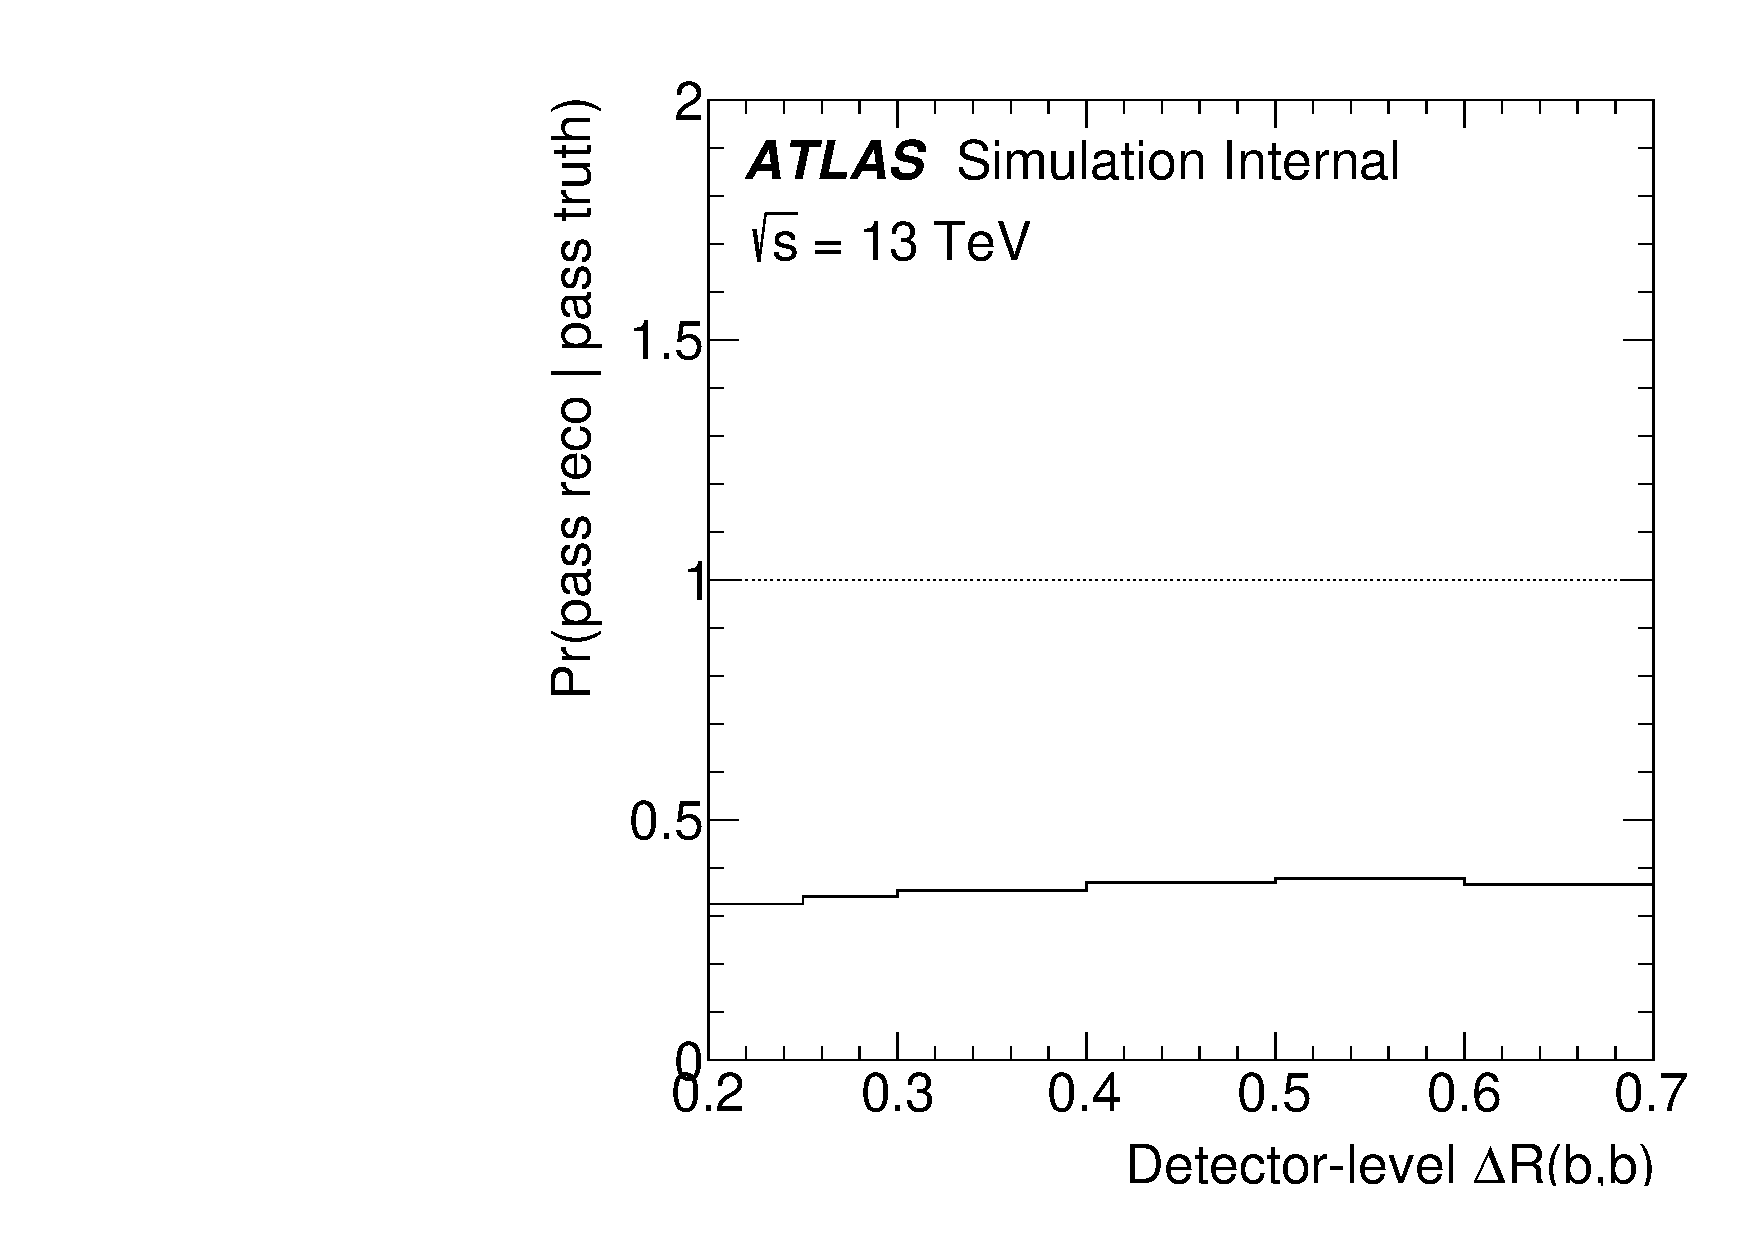
\includegraphics[width=0.45\linewidth]{figures/gbb/Unfolding/dR_effic_factor.pdf}
  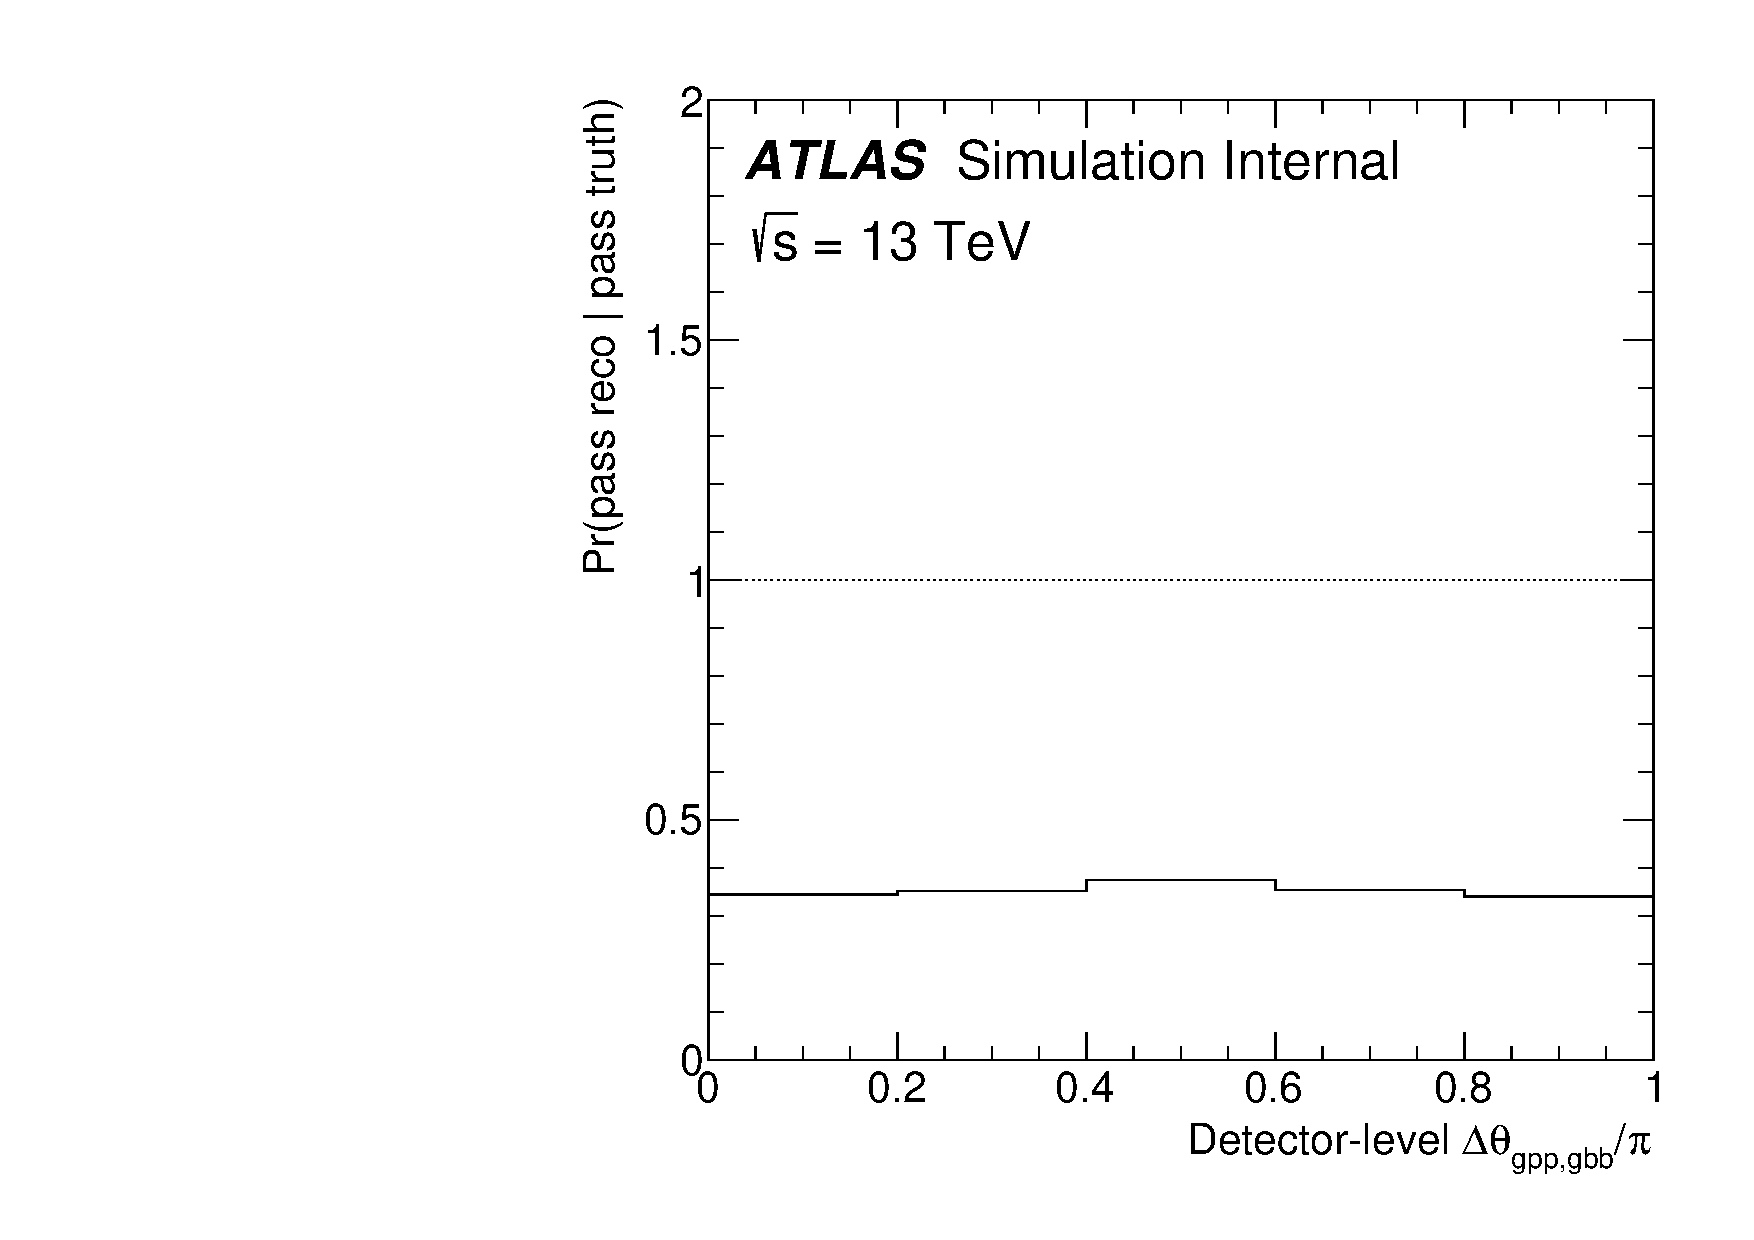
\includegraphics[width=0.45\linewidth]{figures/gbb/Unfolding/dphi_effic_factor.pdf}\\
  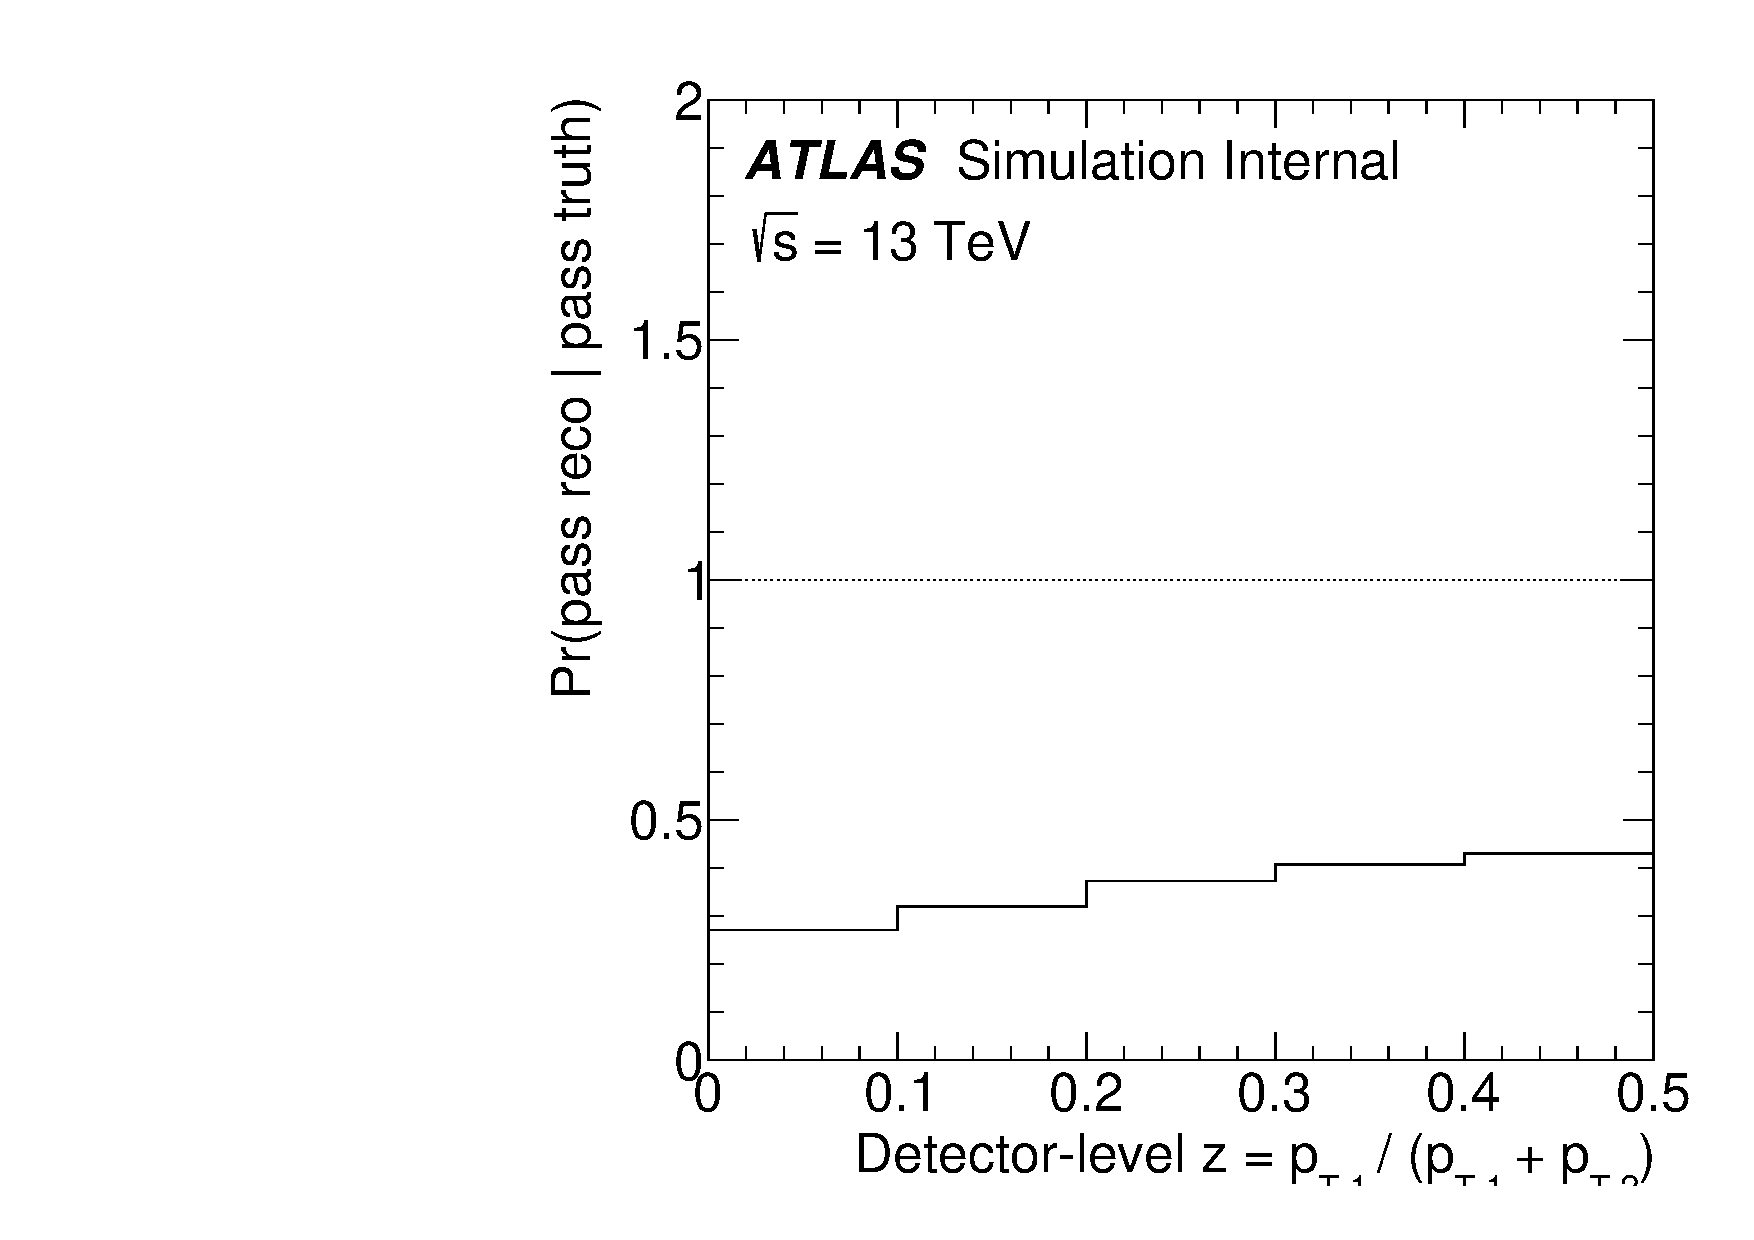
\includegraphics[width=0.45\linewidth]{figures/gbb/Unfolding/ZpT_effic_factor.pdf}
  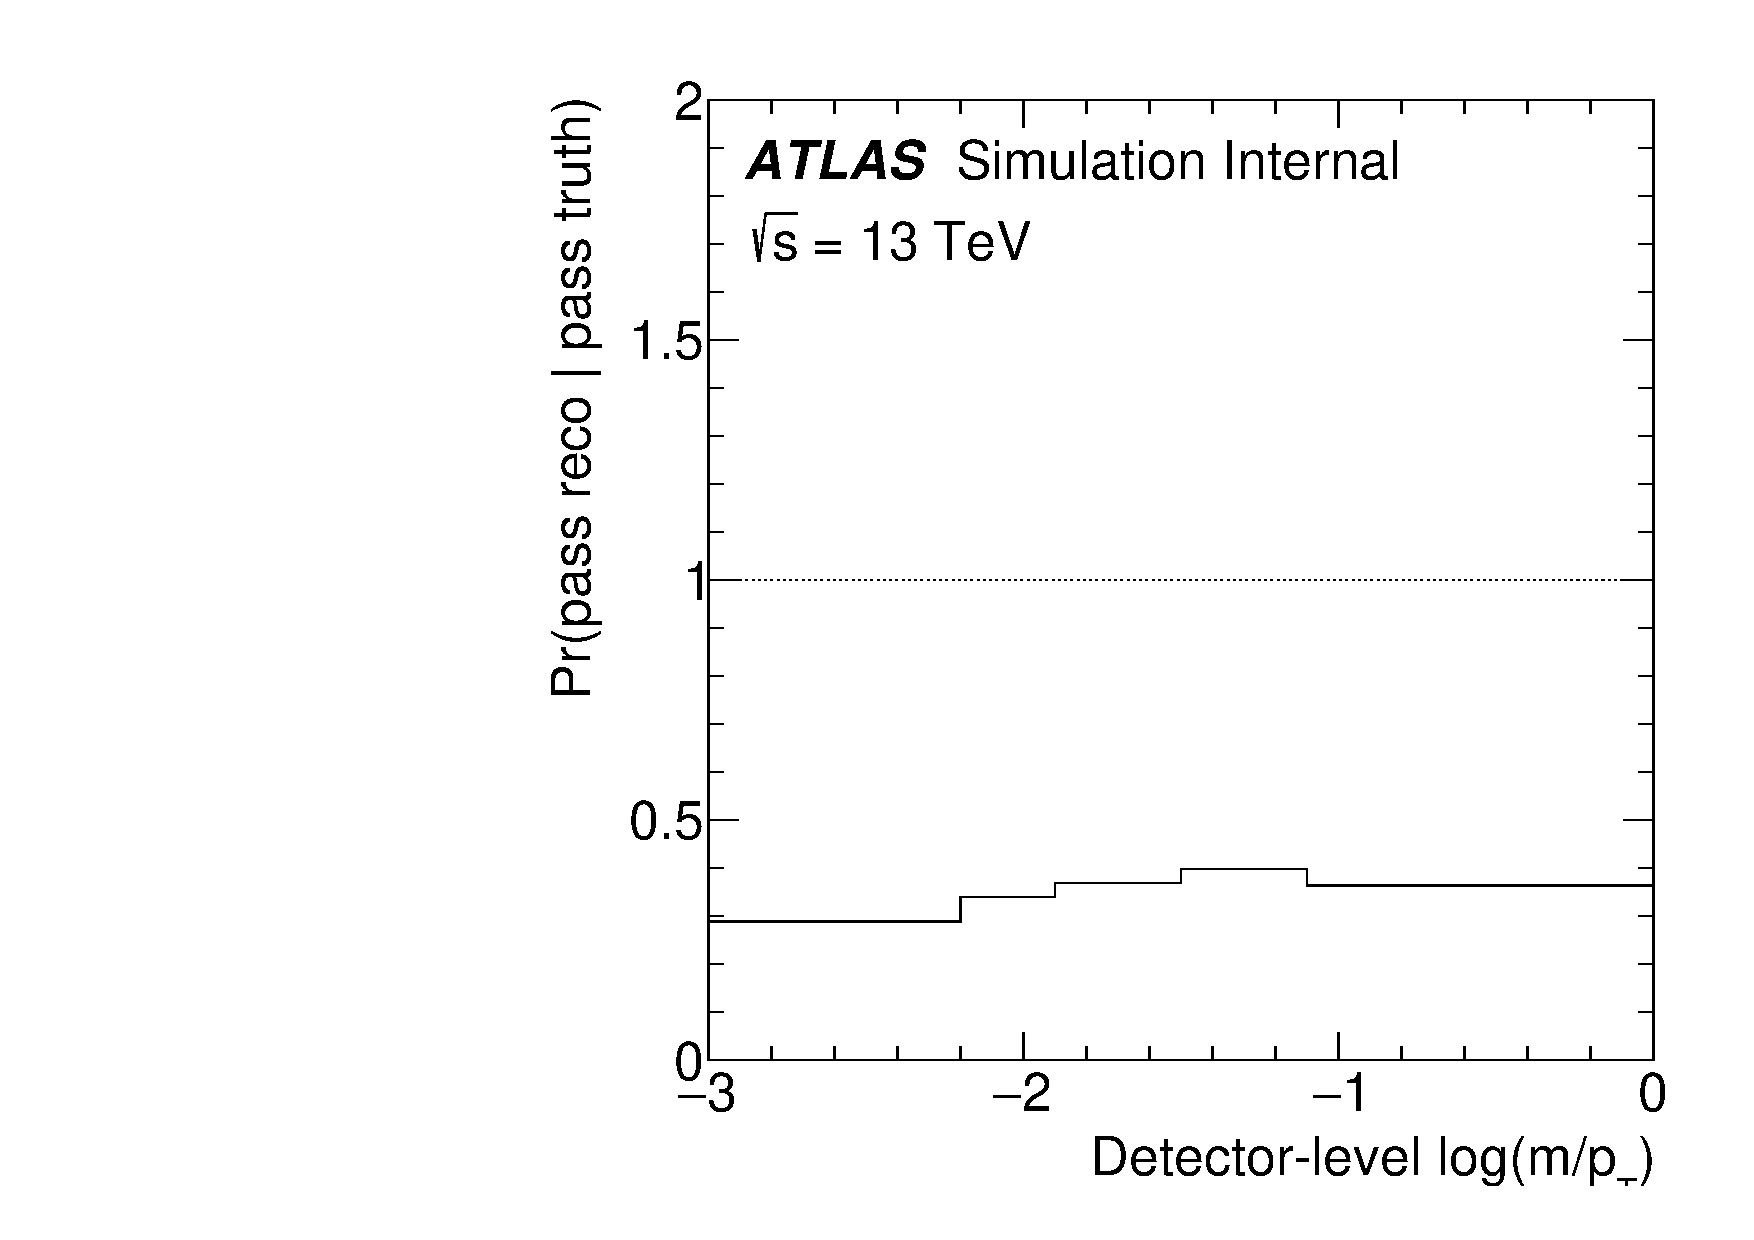
\includegraphics[width=0.45\linewidth]{figures/gbb/Unfolding/fracmasspt_effic_factor.pdf}
\caption[]{The efficiency factors as described in Sec.~\ref{sec:gbb-unfoldingintro}.} 
\label{fig:gbb-acceptance}
\end{center}
\end{figure}

\begin{figure}[htpb!]
\begin{center}
  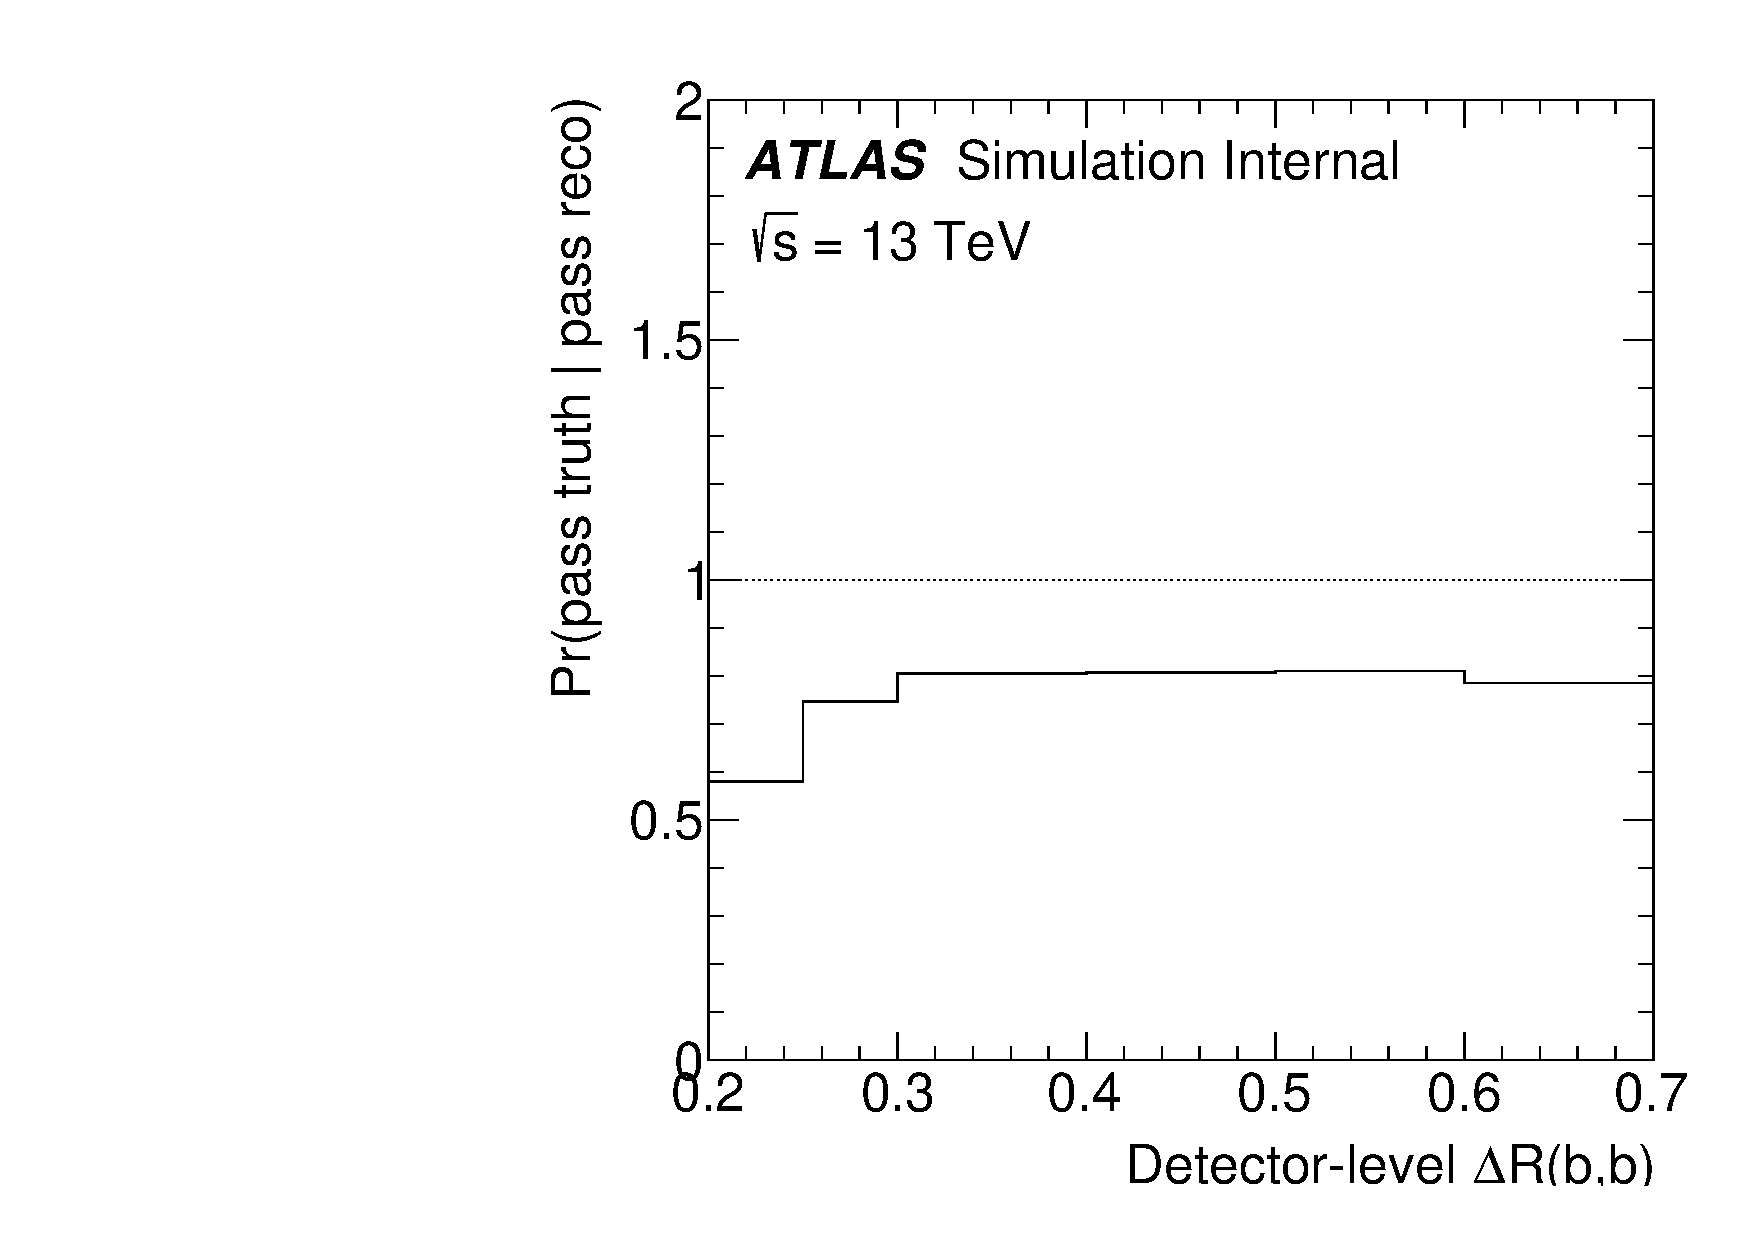
\includegraphics[width=0.45\linewidth]{figures/gbb/Unfolding/dR_fake_factor.pdf}
  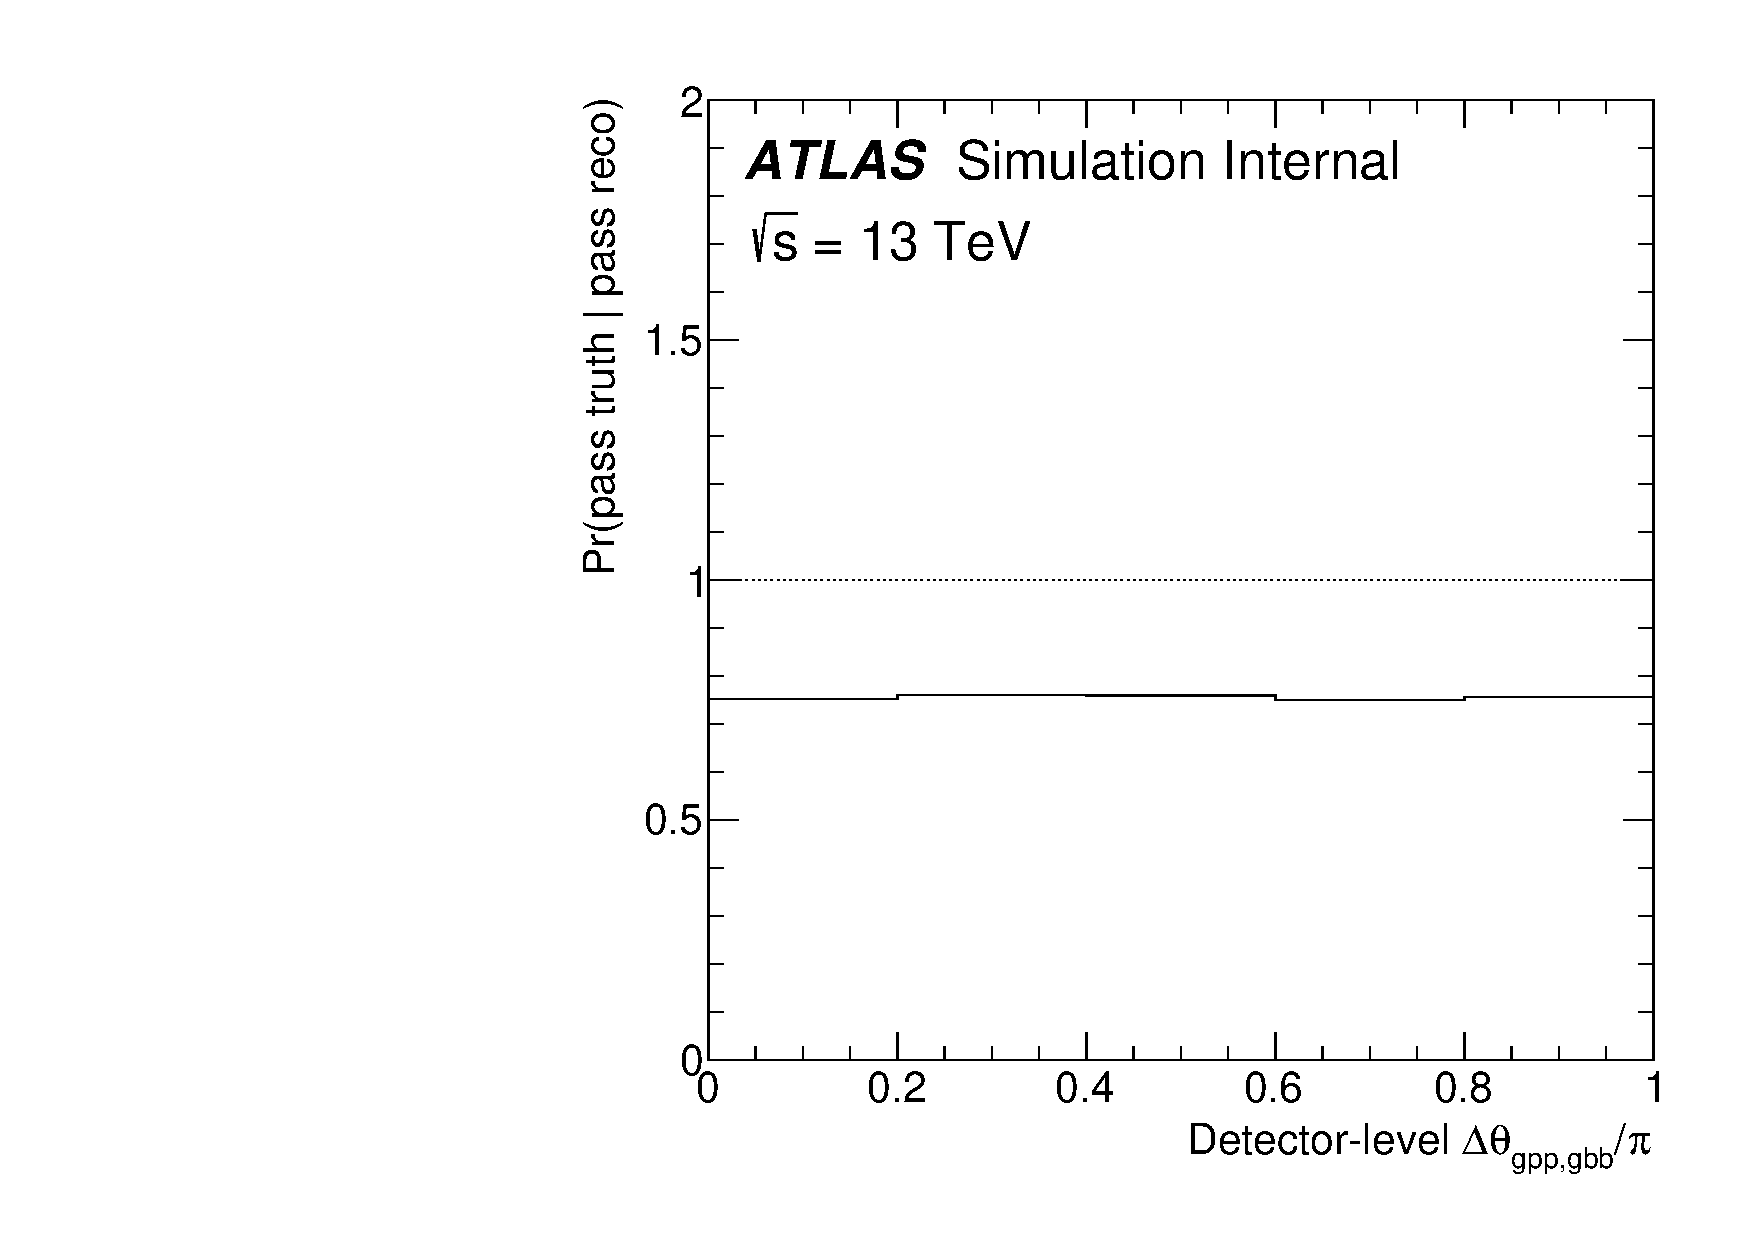
\includegraphics[width=0.45\linewidth]{figures/gbb/Unfolding/dphi_fake_factor.pdf}\\
  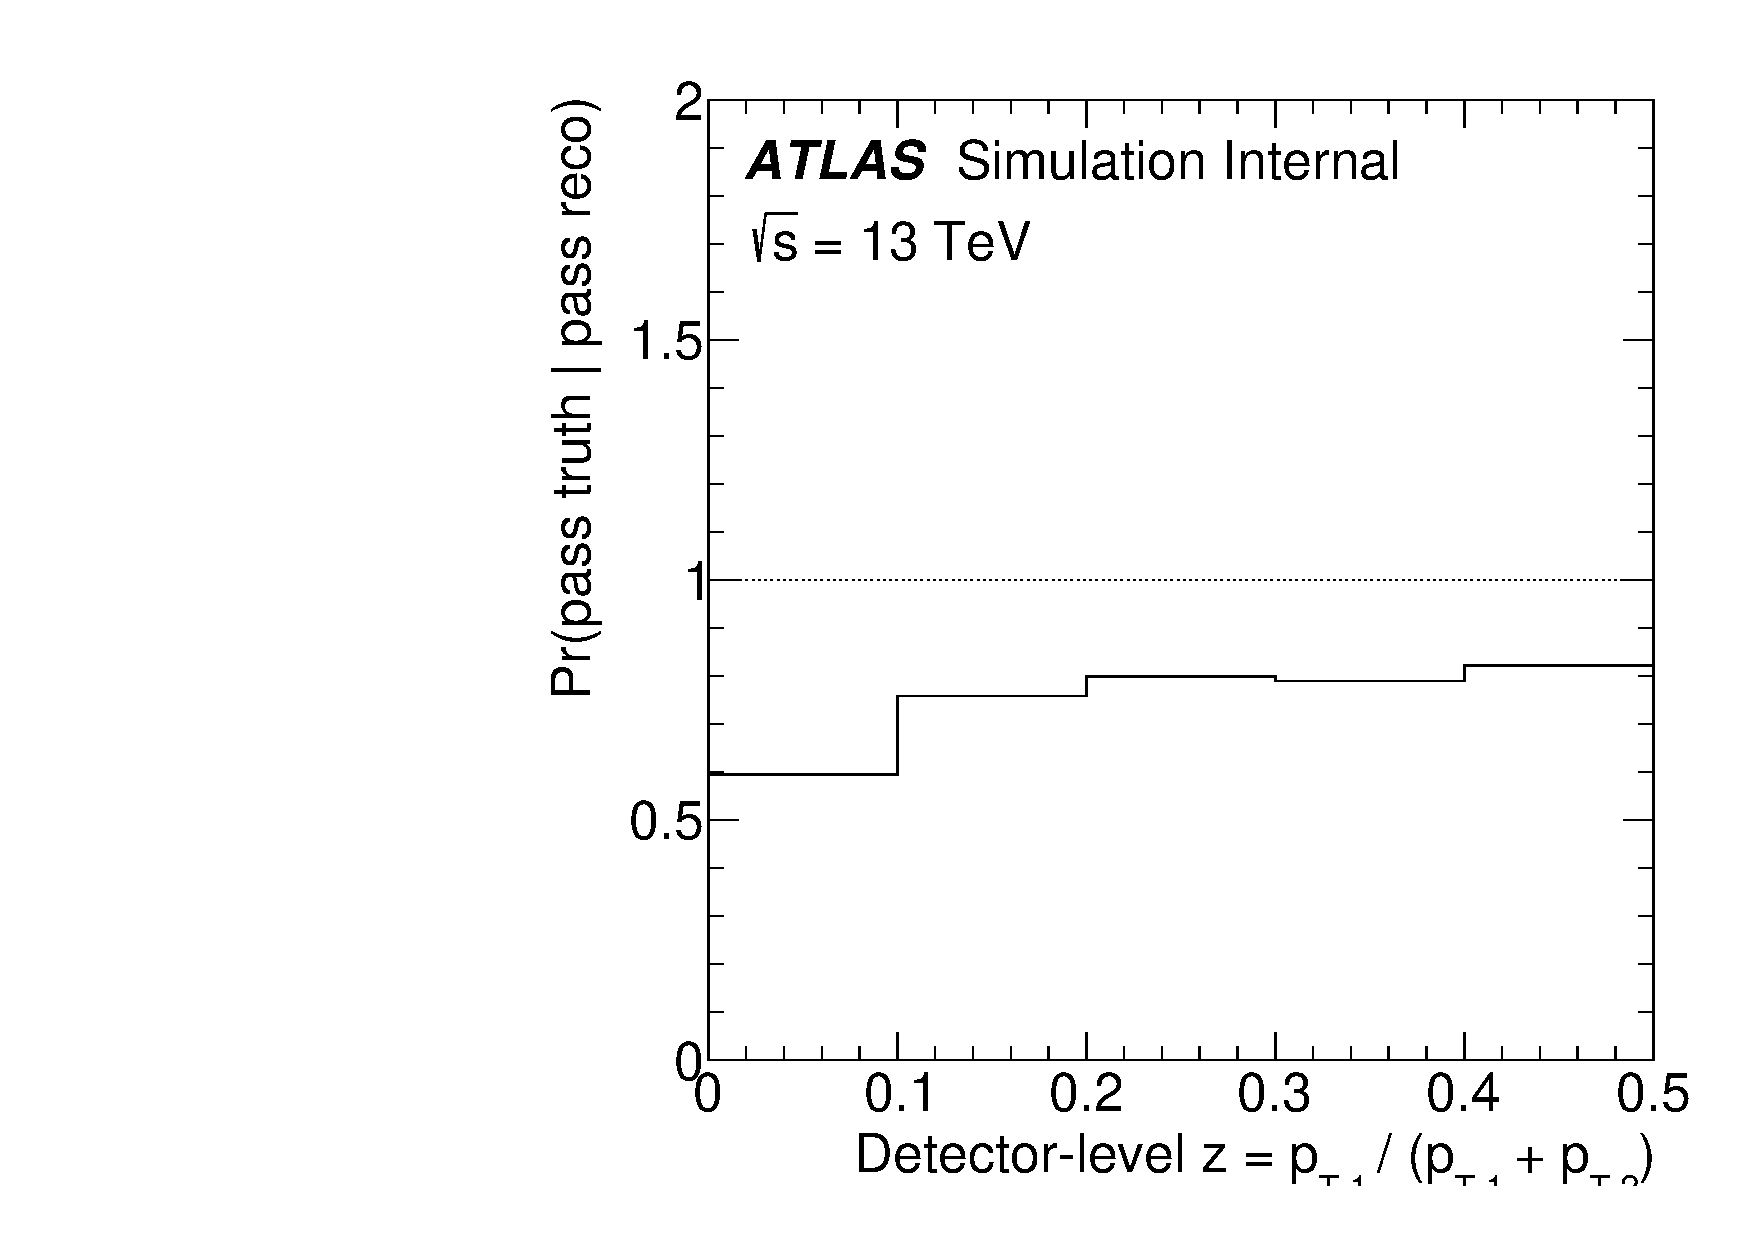
\includegraphics[width=0.45\linewidth]{figures/gbb/Unfolding/ZpT_fake_factor.pdf}
  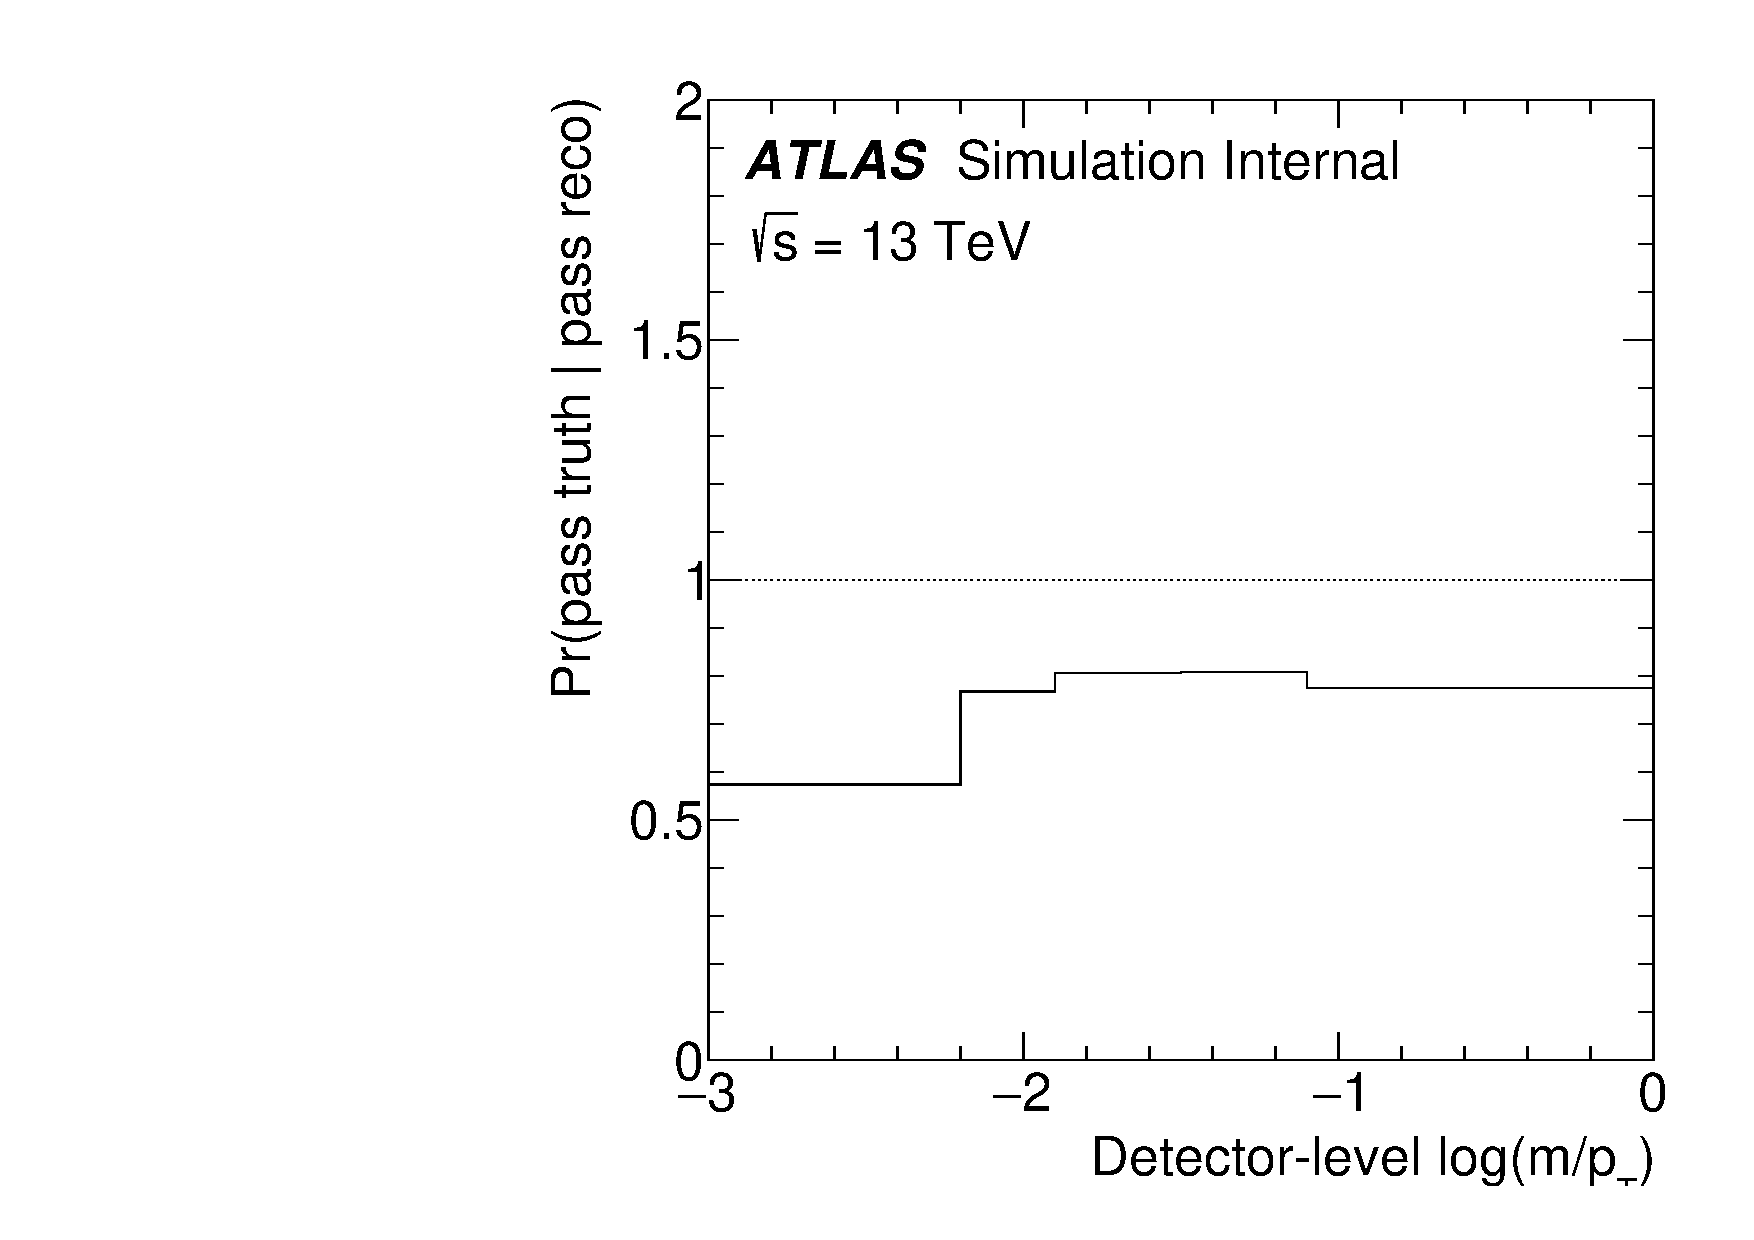
\includegraphics[width=0.45\linewidth]{figures/gbb/Unfolding/fracmasspt_fake_factor.pdf}
\caption[]{The fake factors as described in Sec.~\ref{sec:gbb-unfoldingintro}.} 
\label{fig:gbb-fake}
\end{center}
\end{figure}

\begin{figure}[htpb!]
\begin{center}
  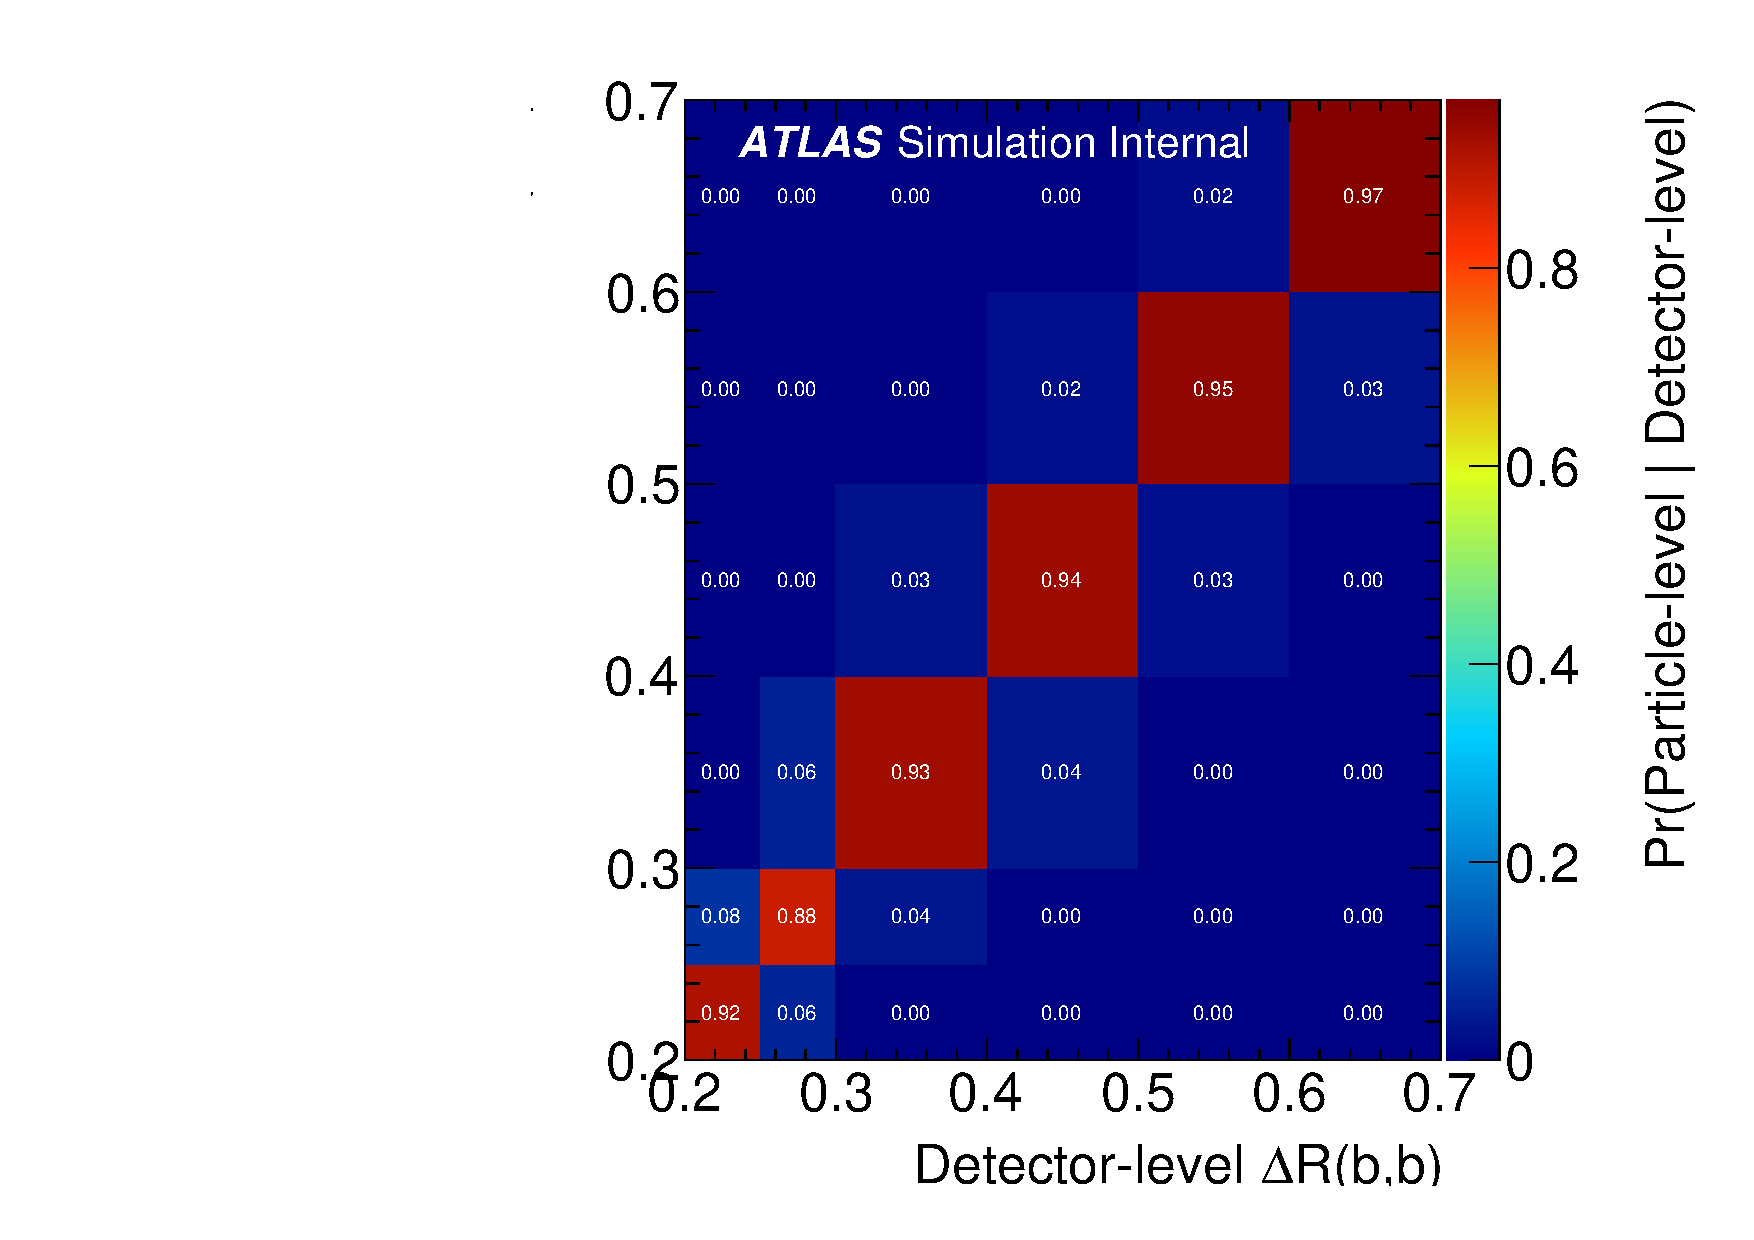
\includegraphics[width=0.45\linewidth]{figures/gbb/Unfolding/dR_ResponseMatrix_x.pdf}
  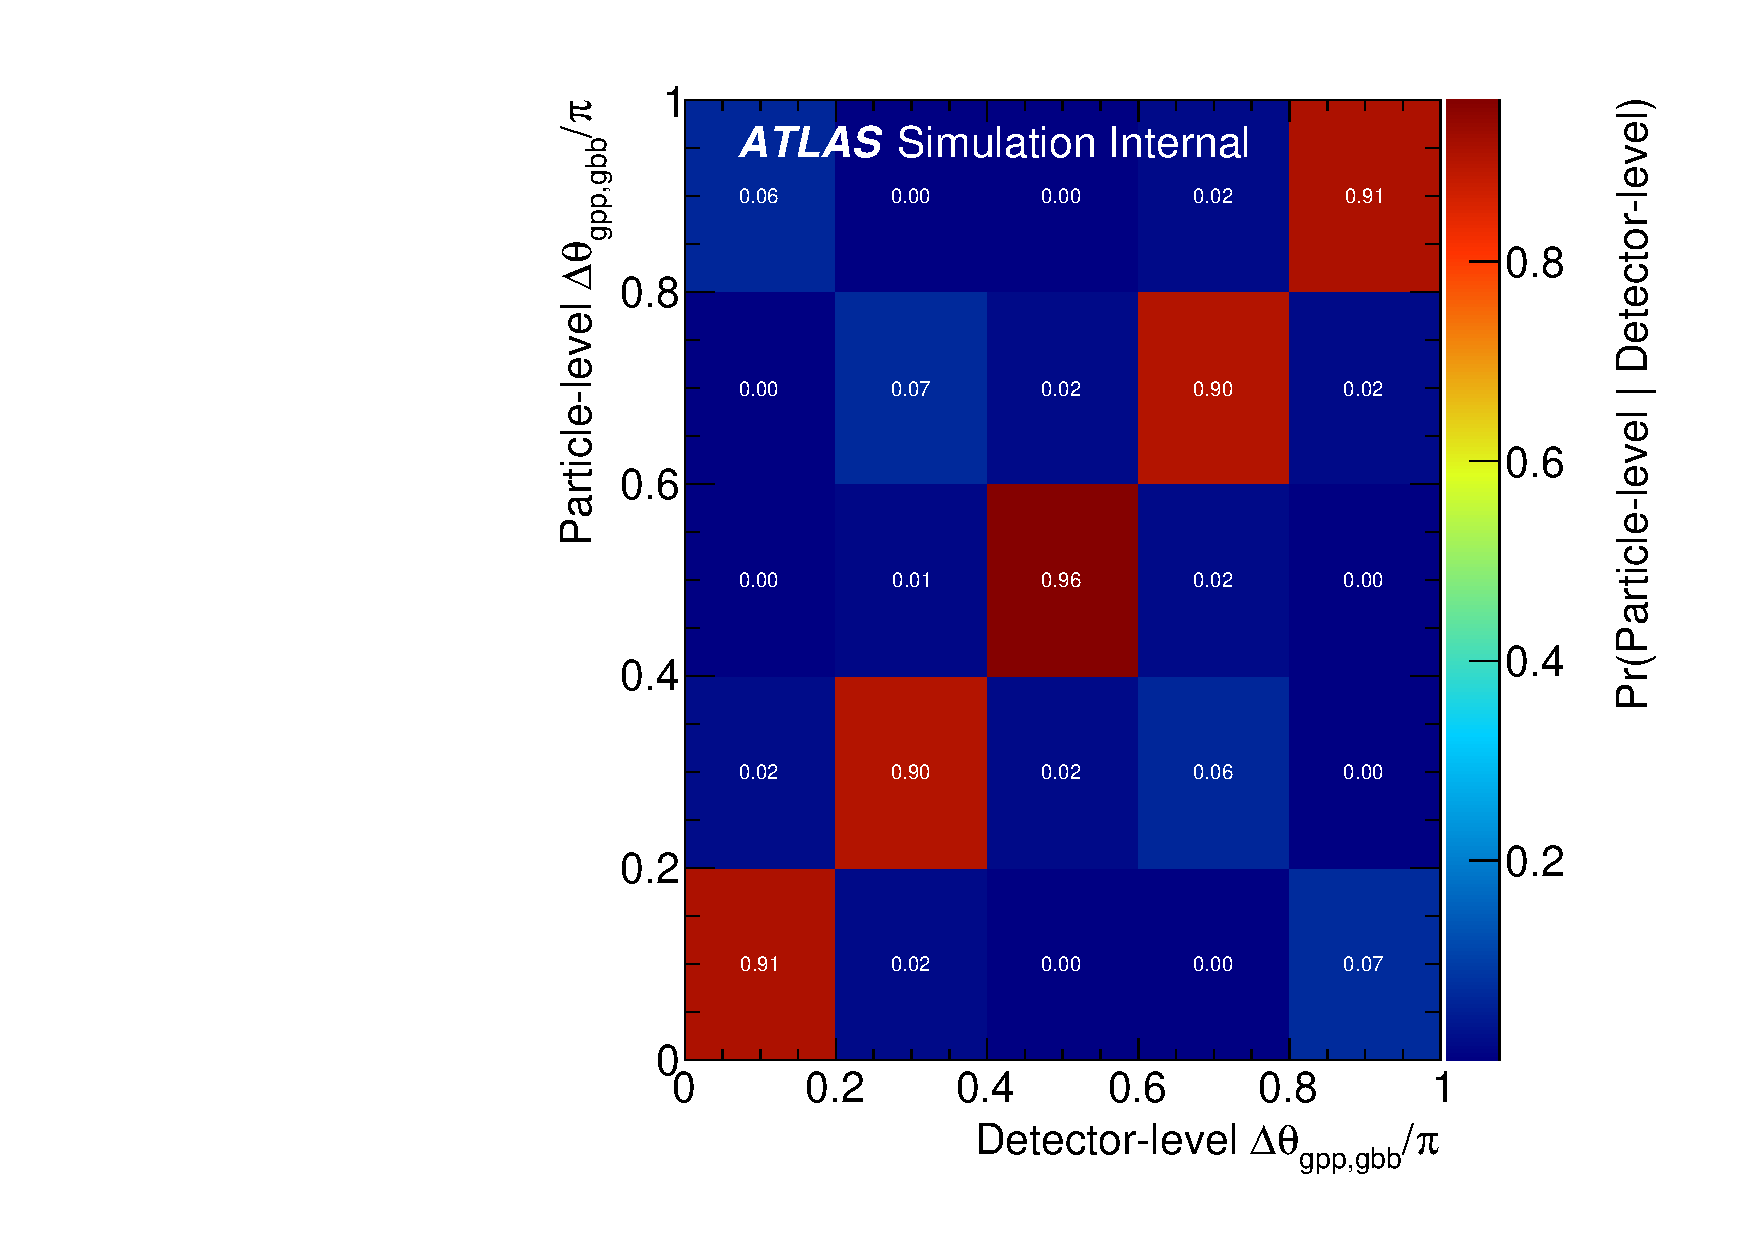
\includegraphics[width=0.45\linewidth]{figures/gbb/Unfolding/dphi_ResponseMatrix_x.pdf}\\
  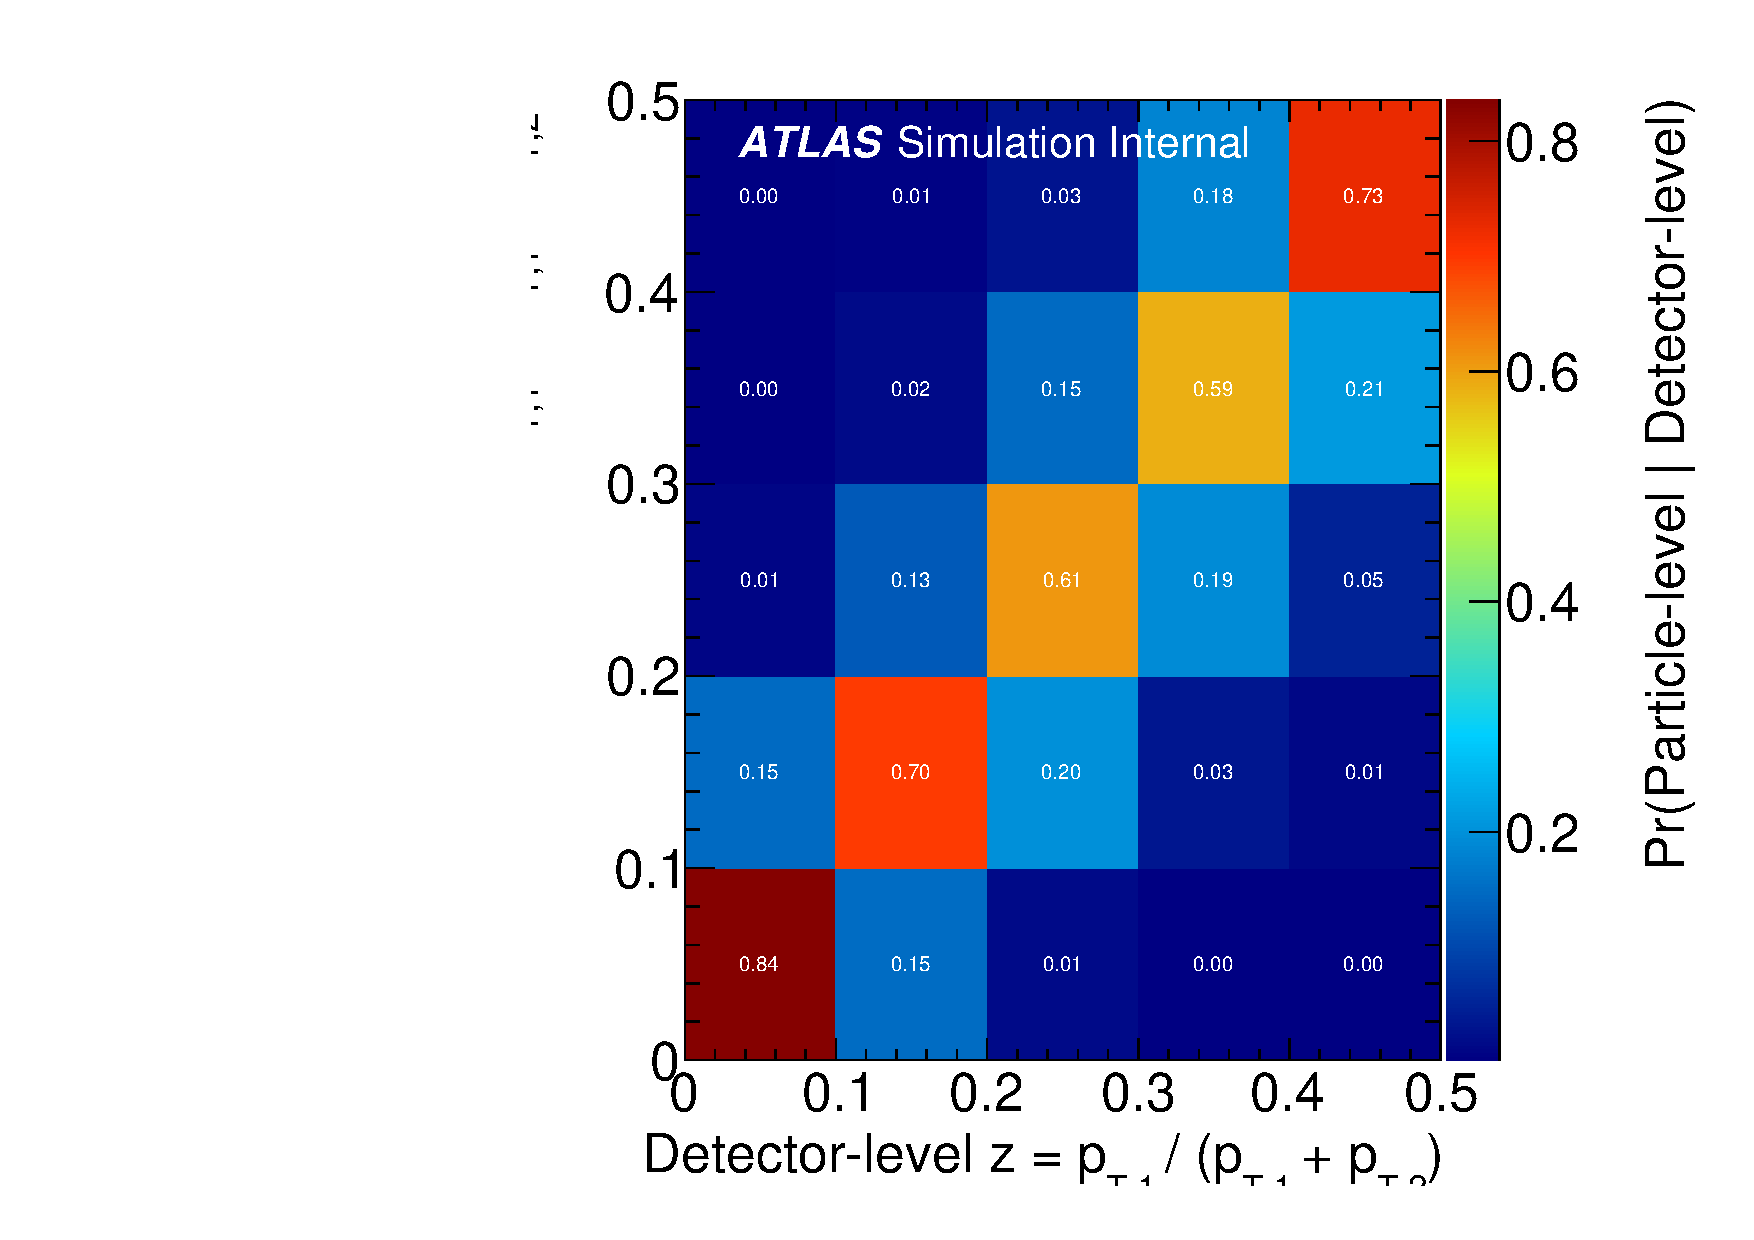
\includegraphics[width=0.45\linewidth]{figures/gbb/Unfolding/ZpT_ResponseMatrix_x.pdf}
  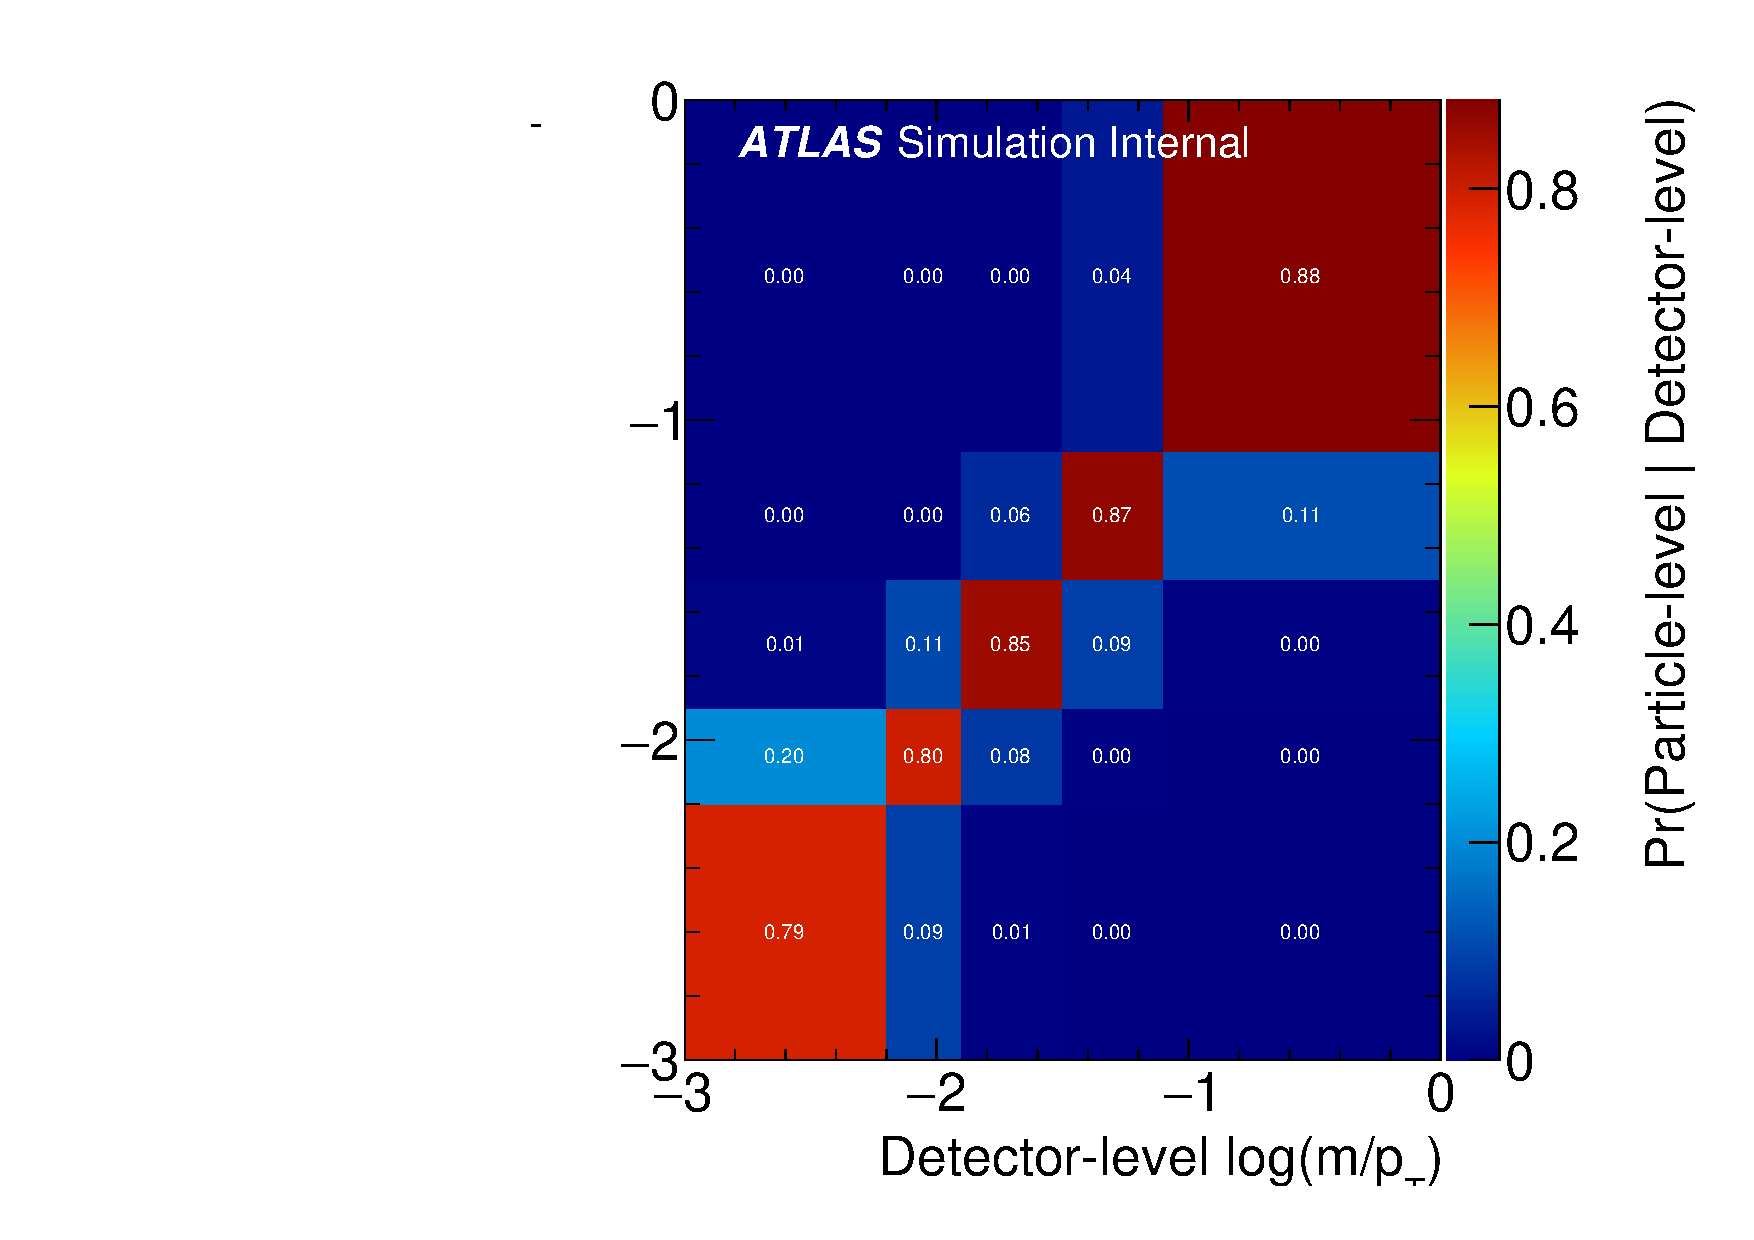
\includegraphics[width=0.45\linewidth]{figures/gbb/Unfolding/fracmasspt_ResponseMatrix_x.pdf}
\caption[]{The unfolding matrices.  } 
\label{fig:gbb-responsematrix1}
\end{center}
\end{figure}

\begin{figure}[htpb!]
\begin{center}
  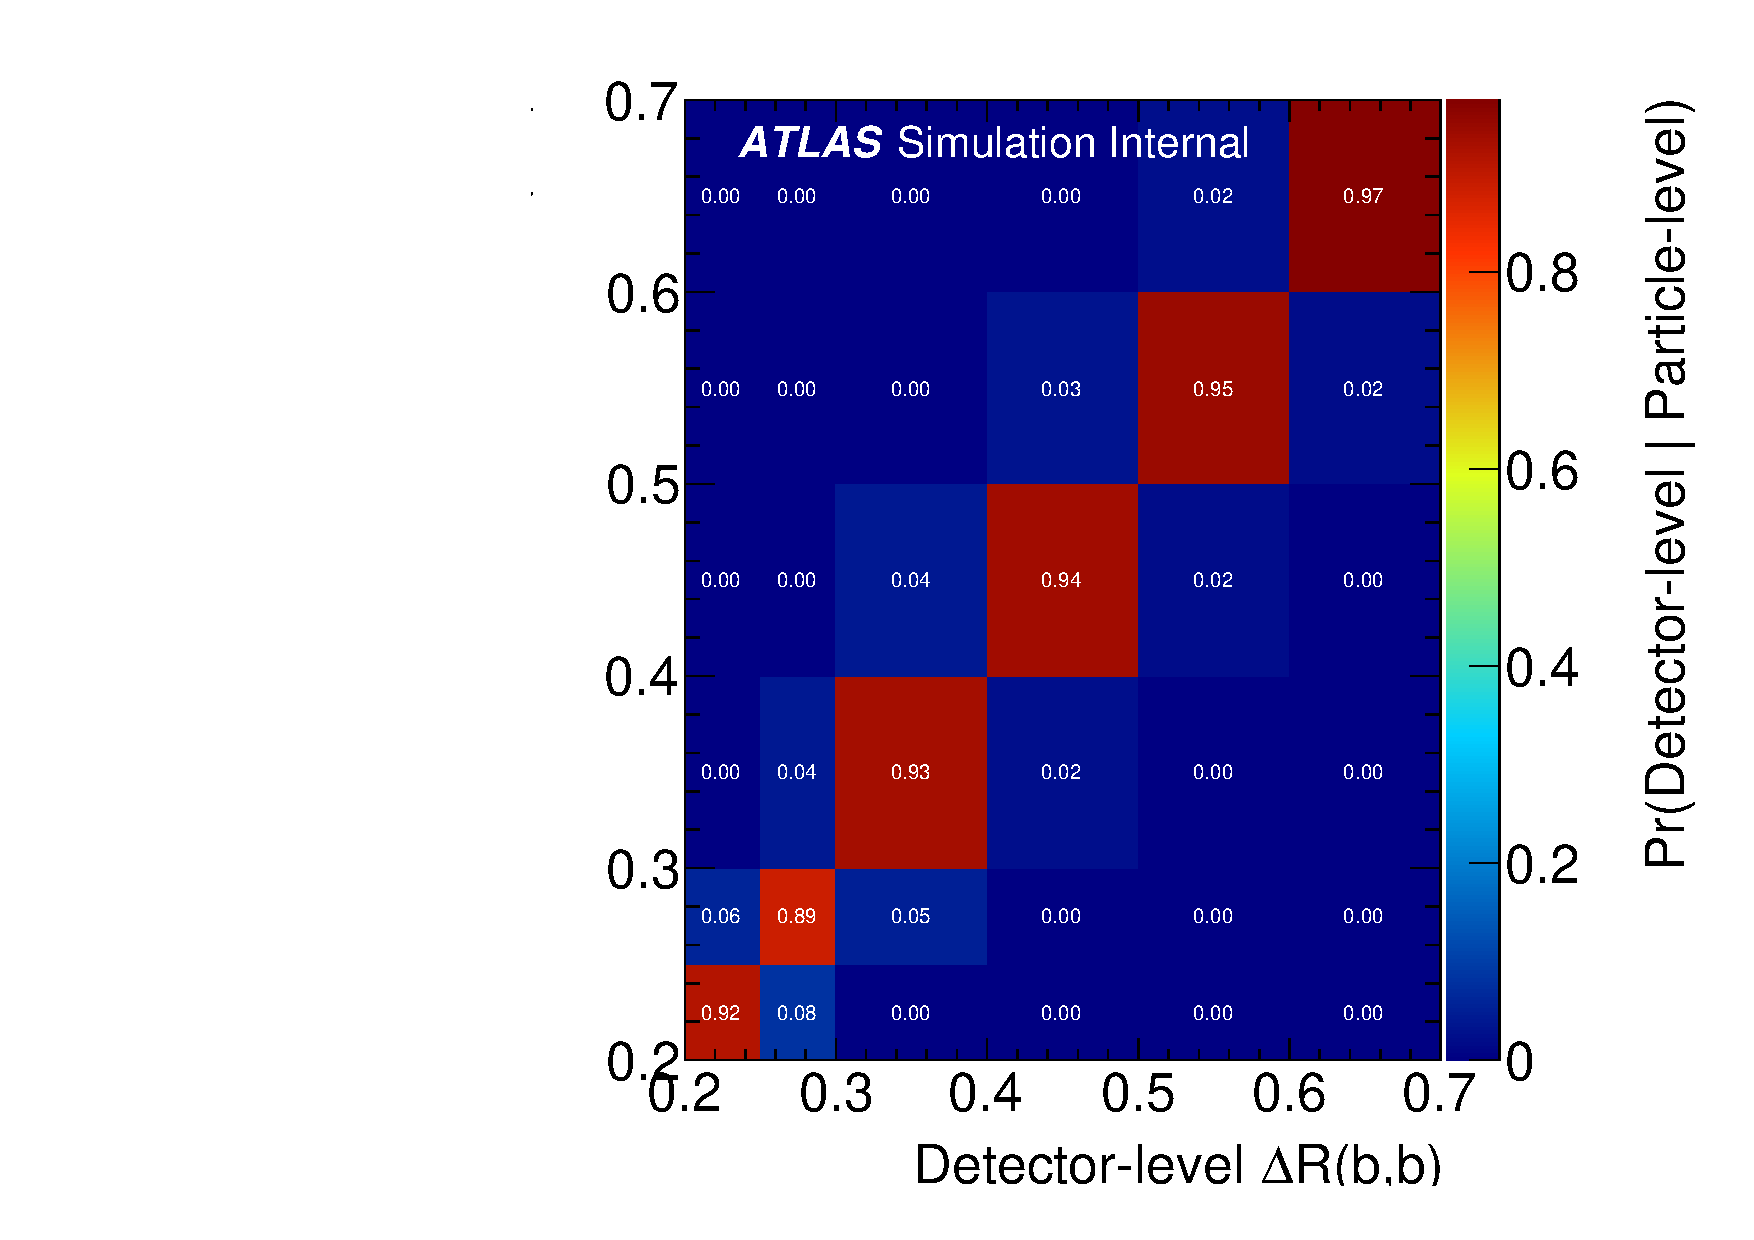
\includegraphics[width=0.45\linewidth]{figures/gbb/Unfolding/dR_ResponseMatrix_y.pdf}
  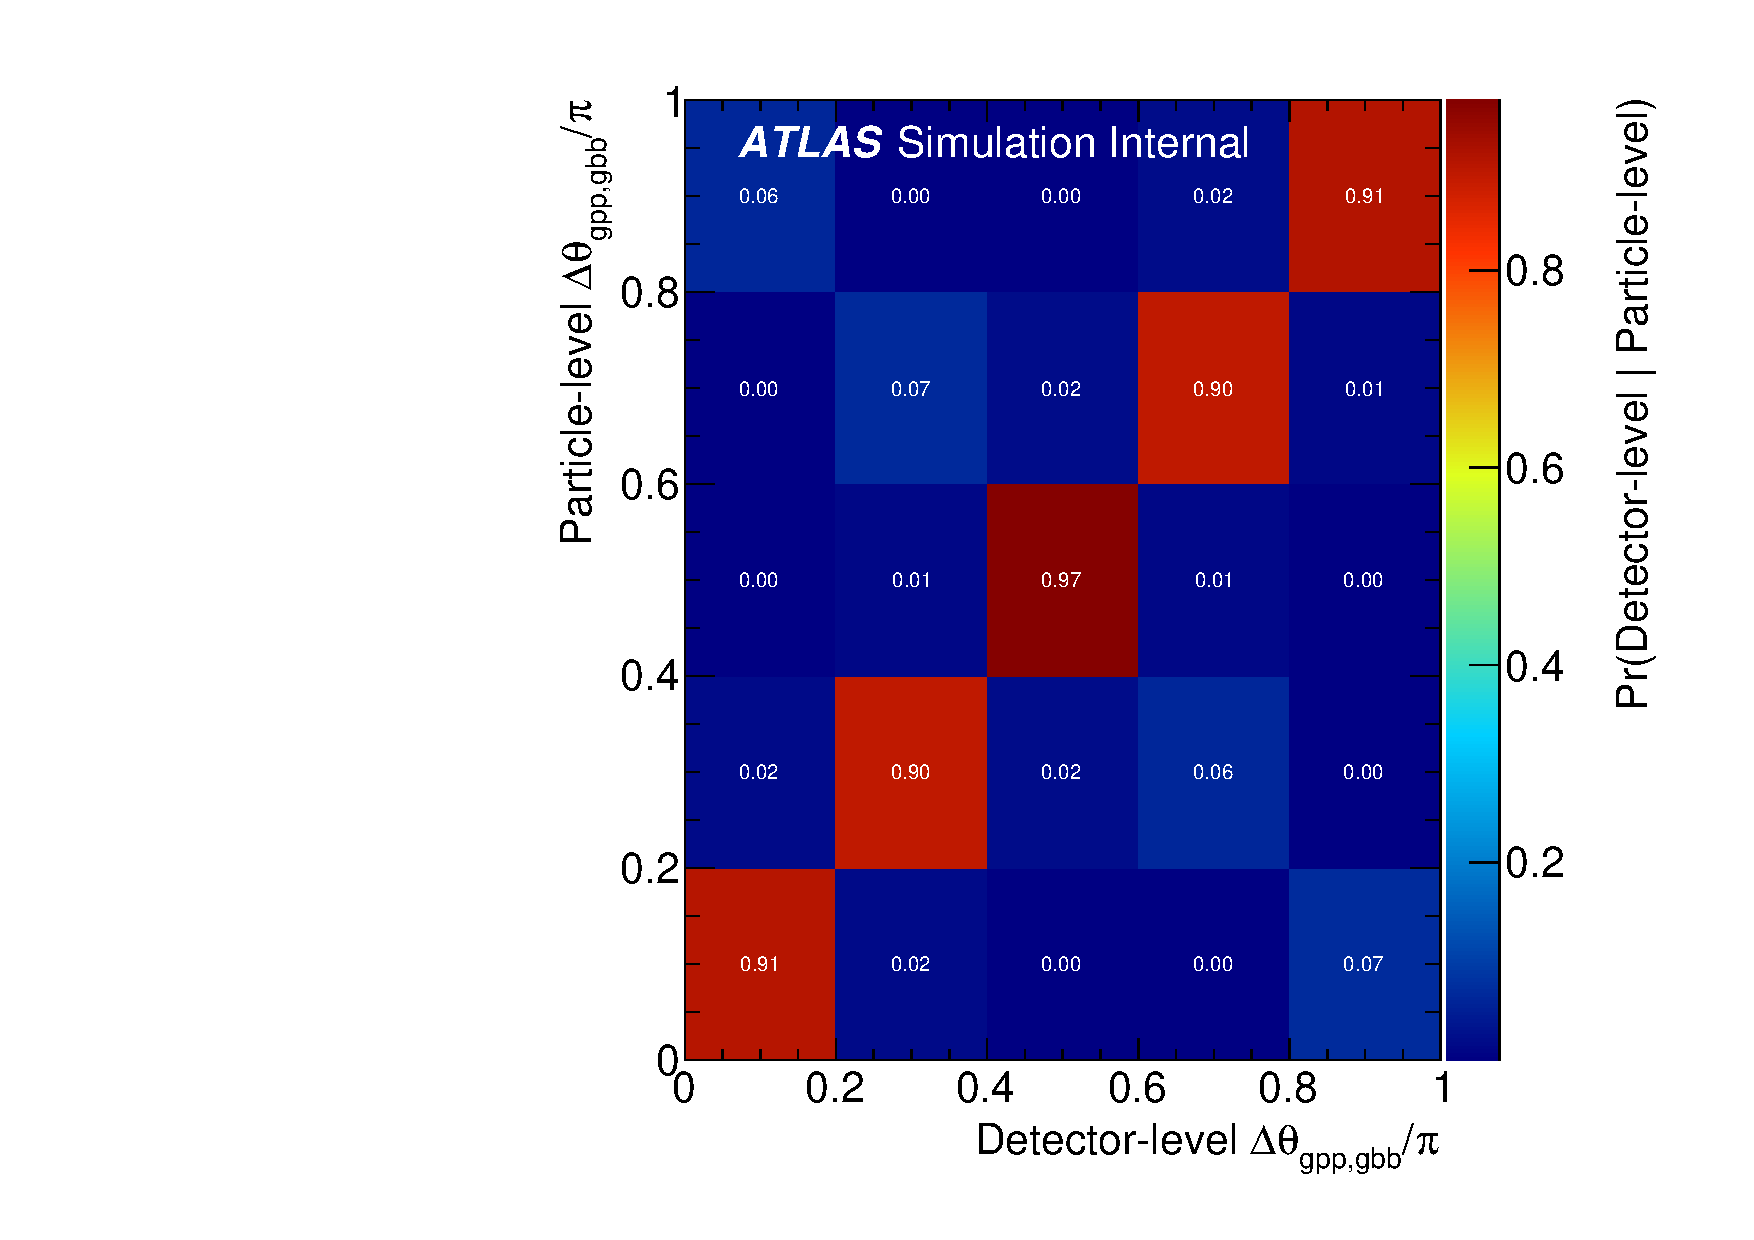
\includegraphics[width=0.45\linewidth]{figures/gbb/Unfolding/dphi_ResponseMatrix_y.pdf}\\
  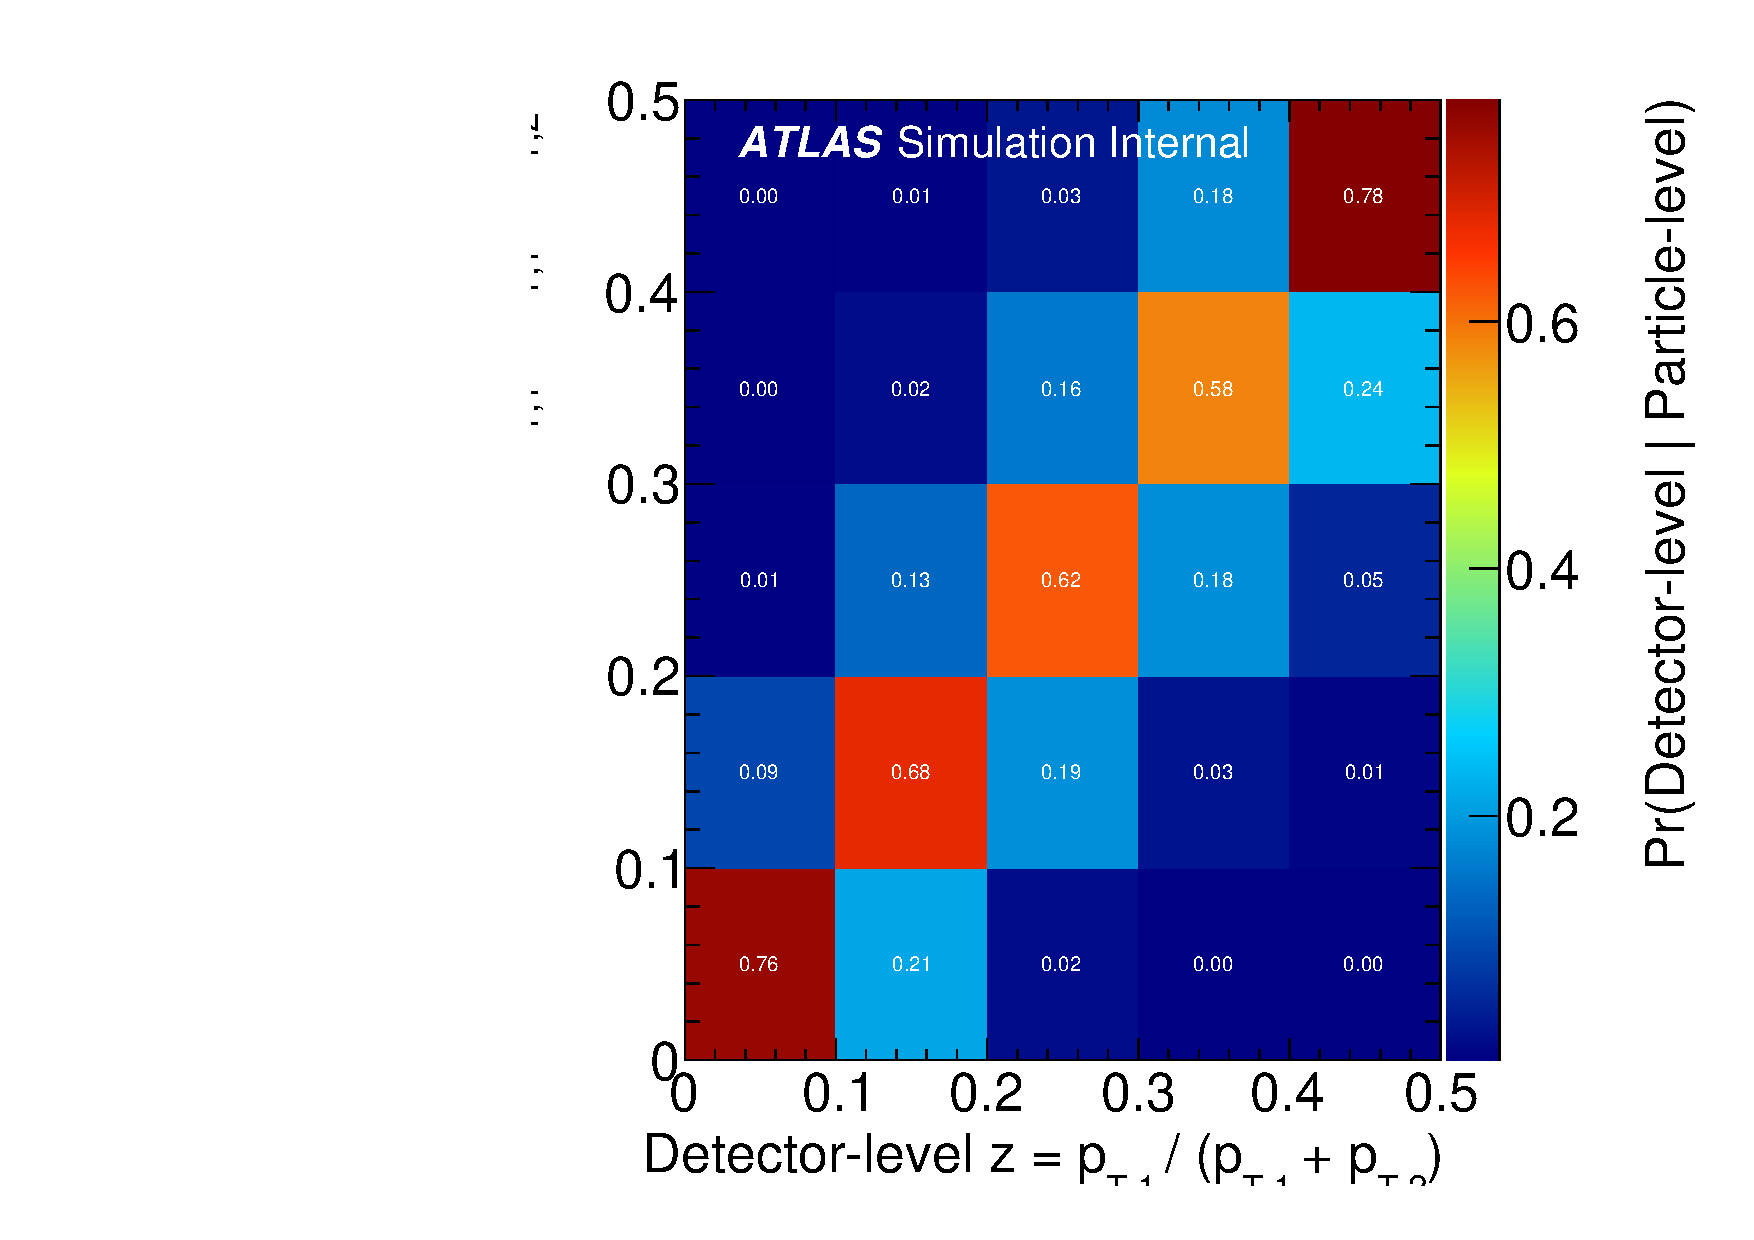
\includegraphics[width=0.45\linewidth]{figures/gbb/Unfolding/ZpT_ResponseMatrix_y.pdf}
  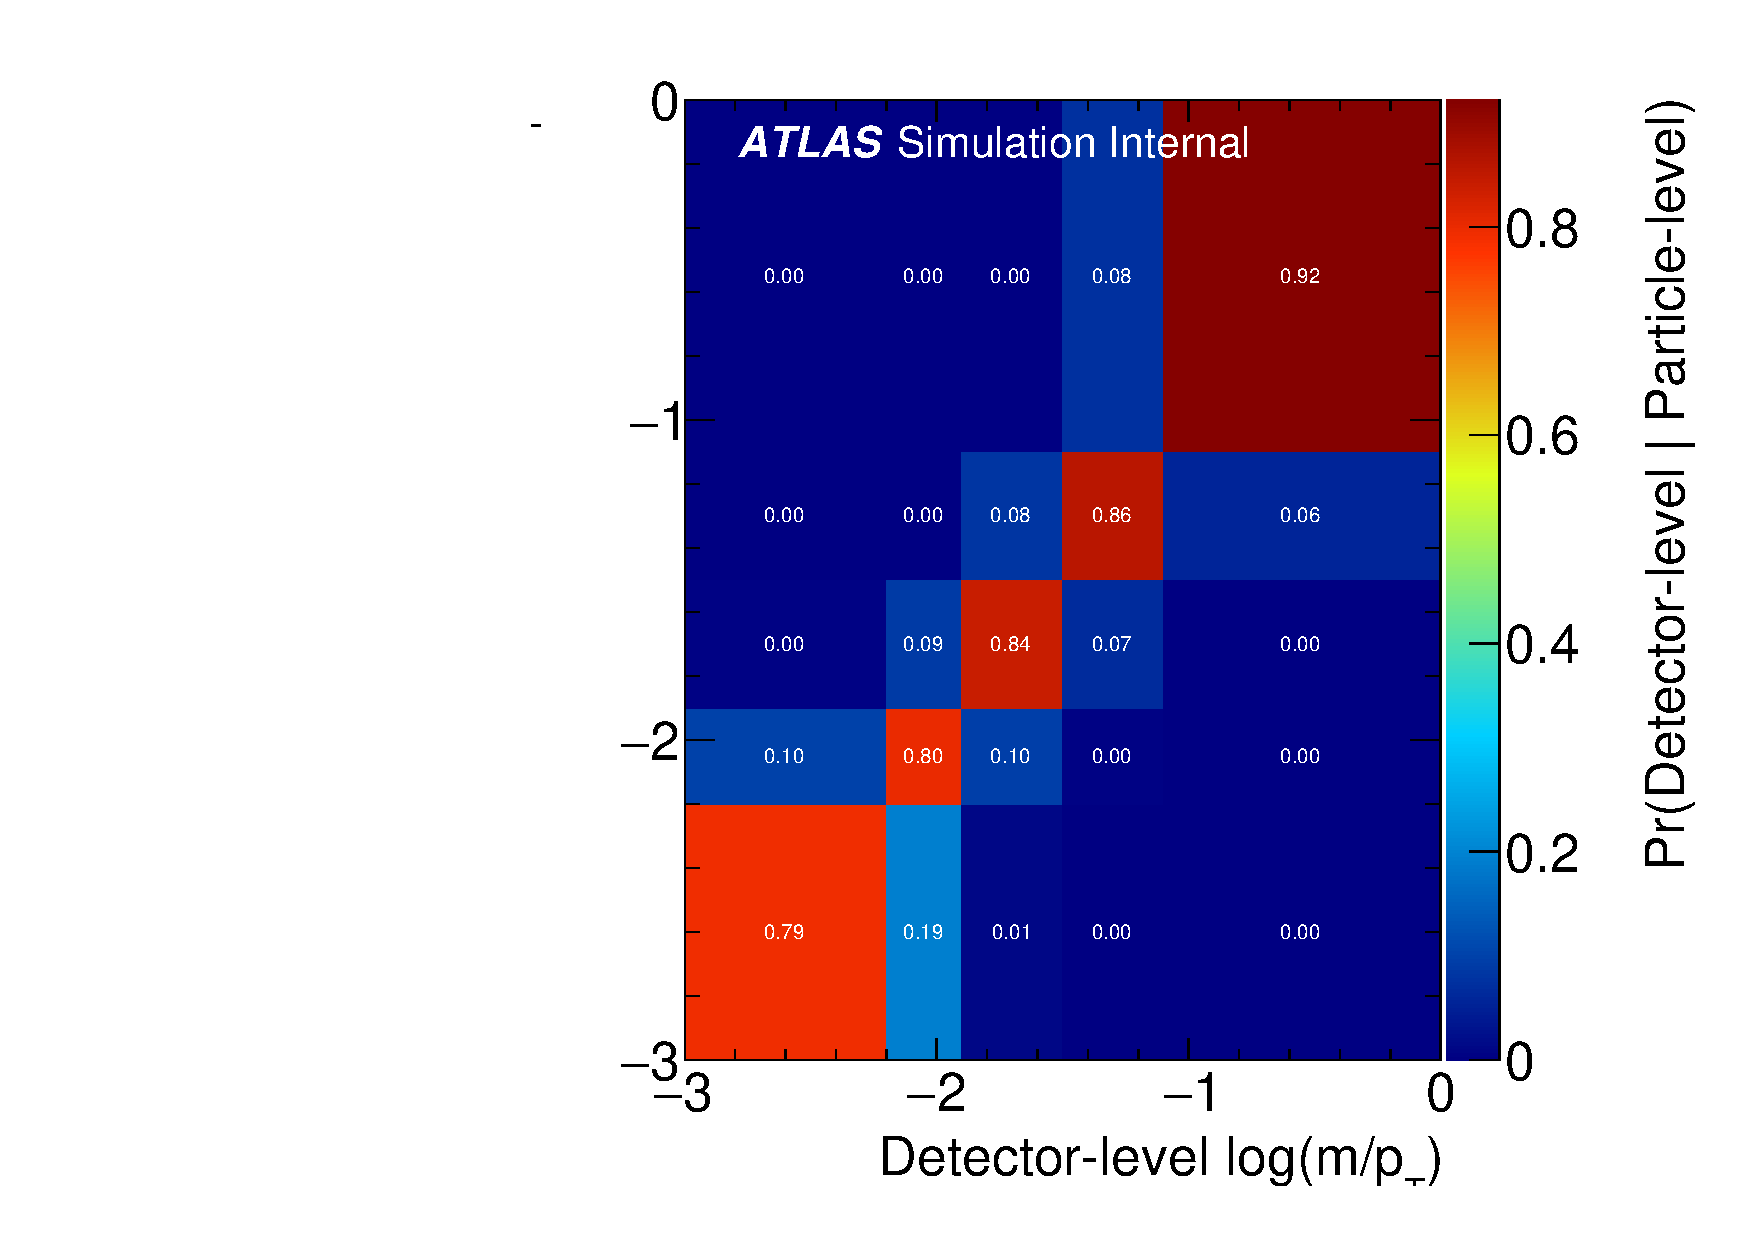
\includegraphics[width=0.45\linewidth]{figures/gbb/Unfolding/fracmasspt_ResponseMatrix_y.pdf}
\caption[]{The folding matrices.  } 
\label{fig:gbb-responsematrix2}
\end{center}
\end{figure}

\clearpage

\subsection{Technical closure}
\label{sec:gbb-unfolding:technicalclosure}

As a technical check of the unfolding procedure, Fig.~\ref{fig:gbb-technicalclosure} shows that the method closes when unfolding Pythia with itself.

\begin{figure}[htpb!]
\begin{center}
  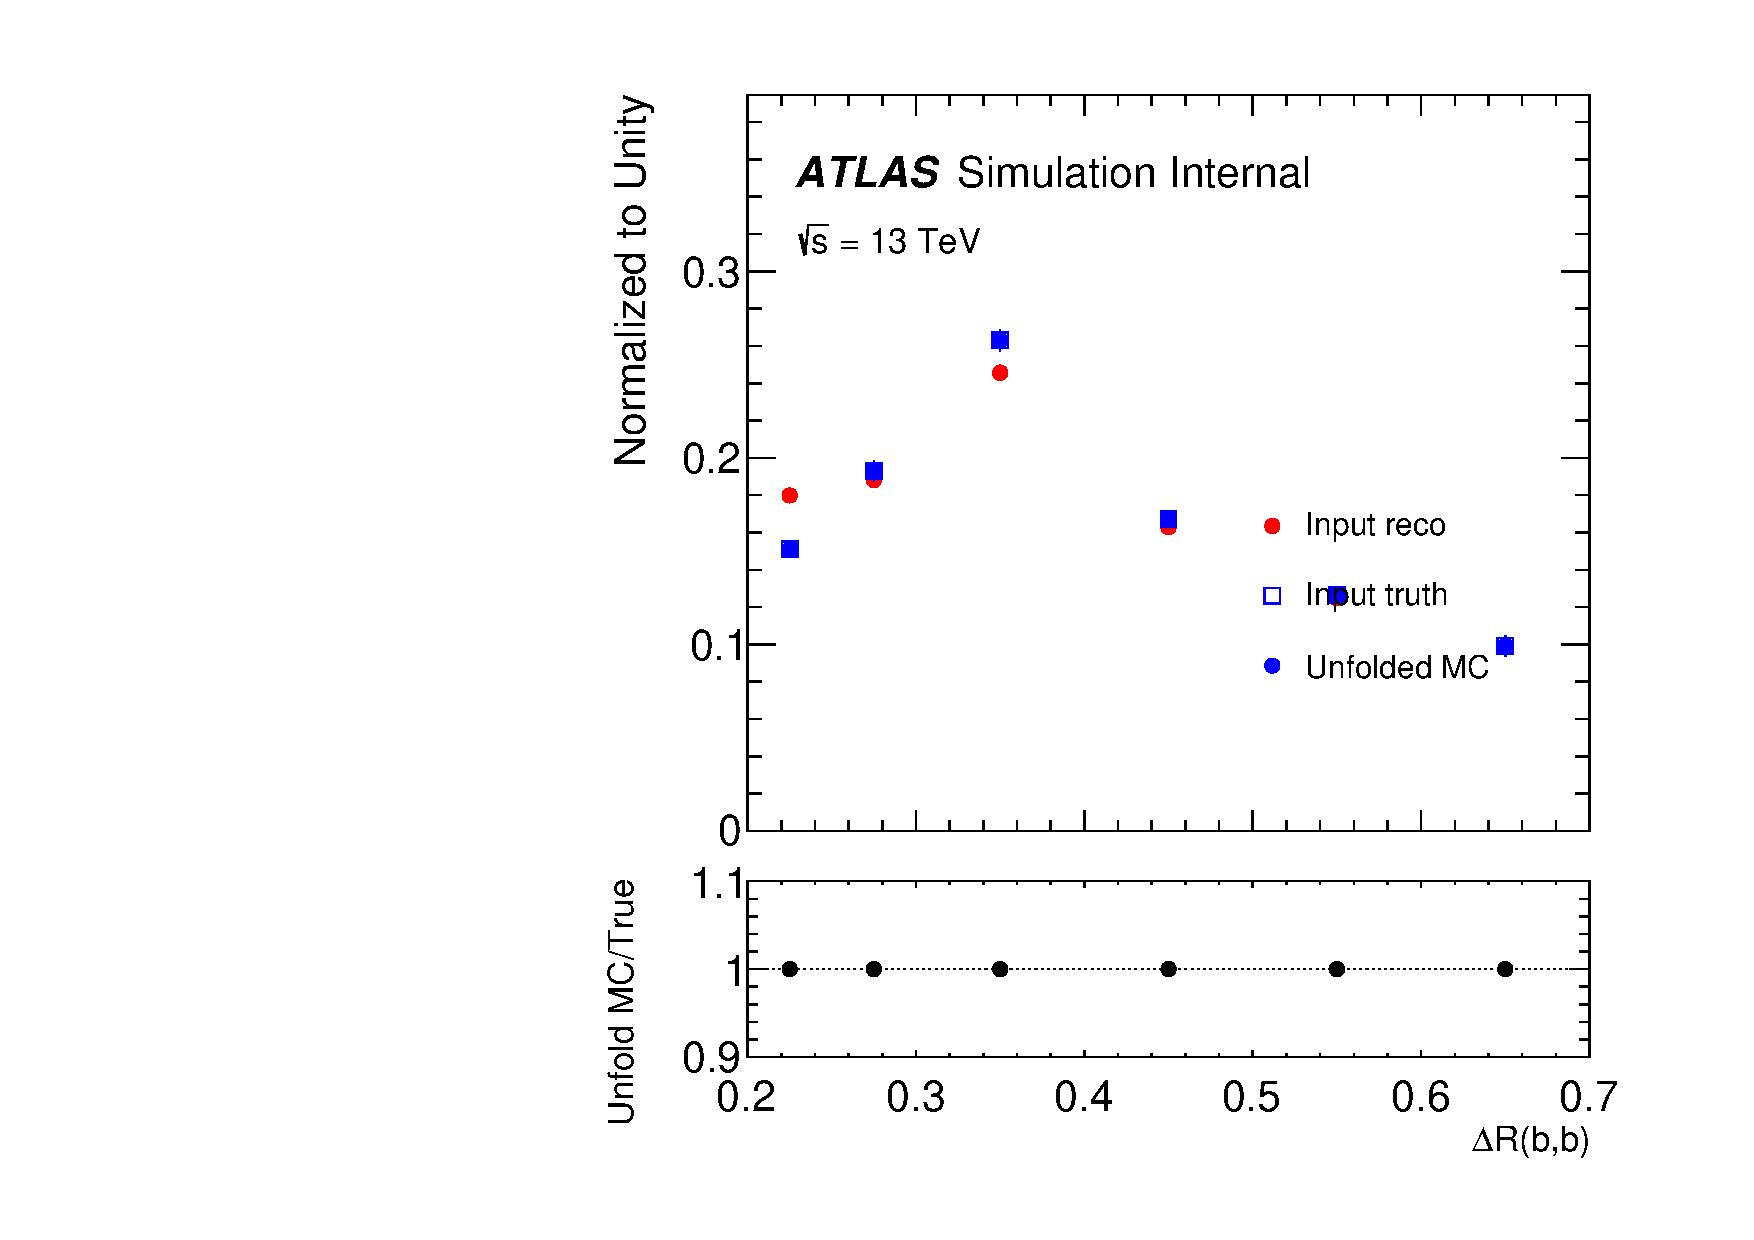
\includegraphics[width=0.45\linewidth]{figures/gbb/Unfolding/dR_technical_closure.pdf}
  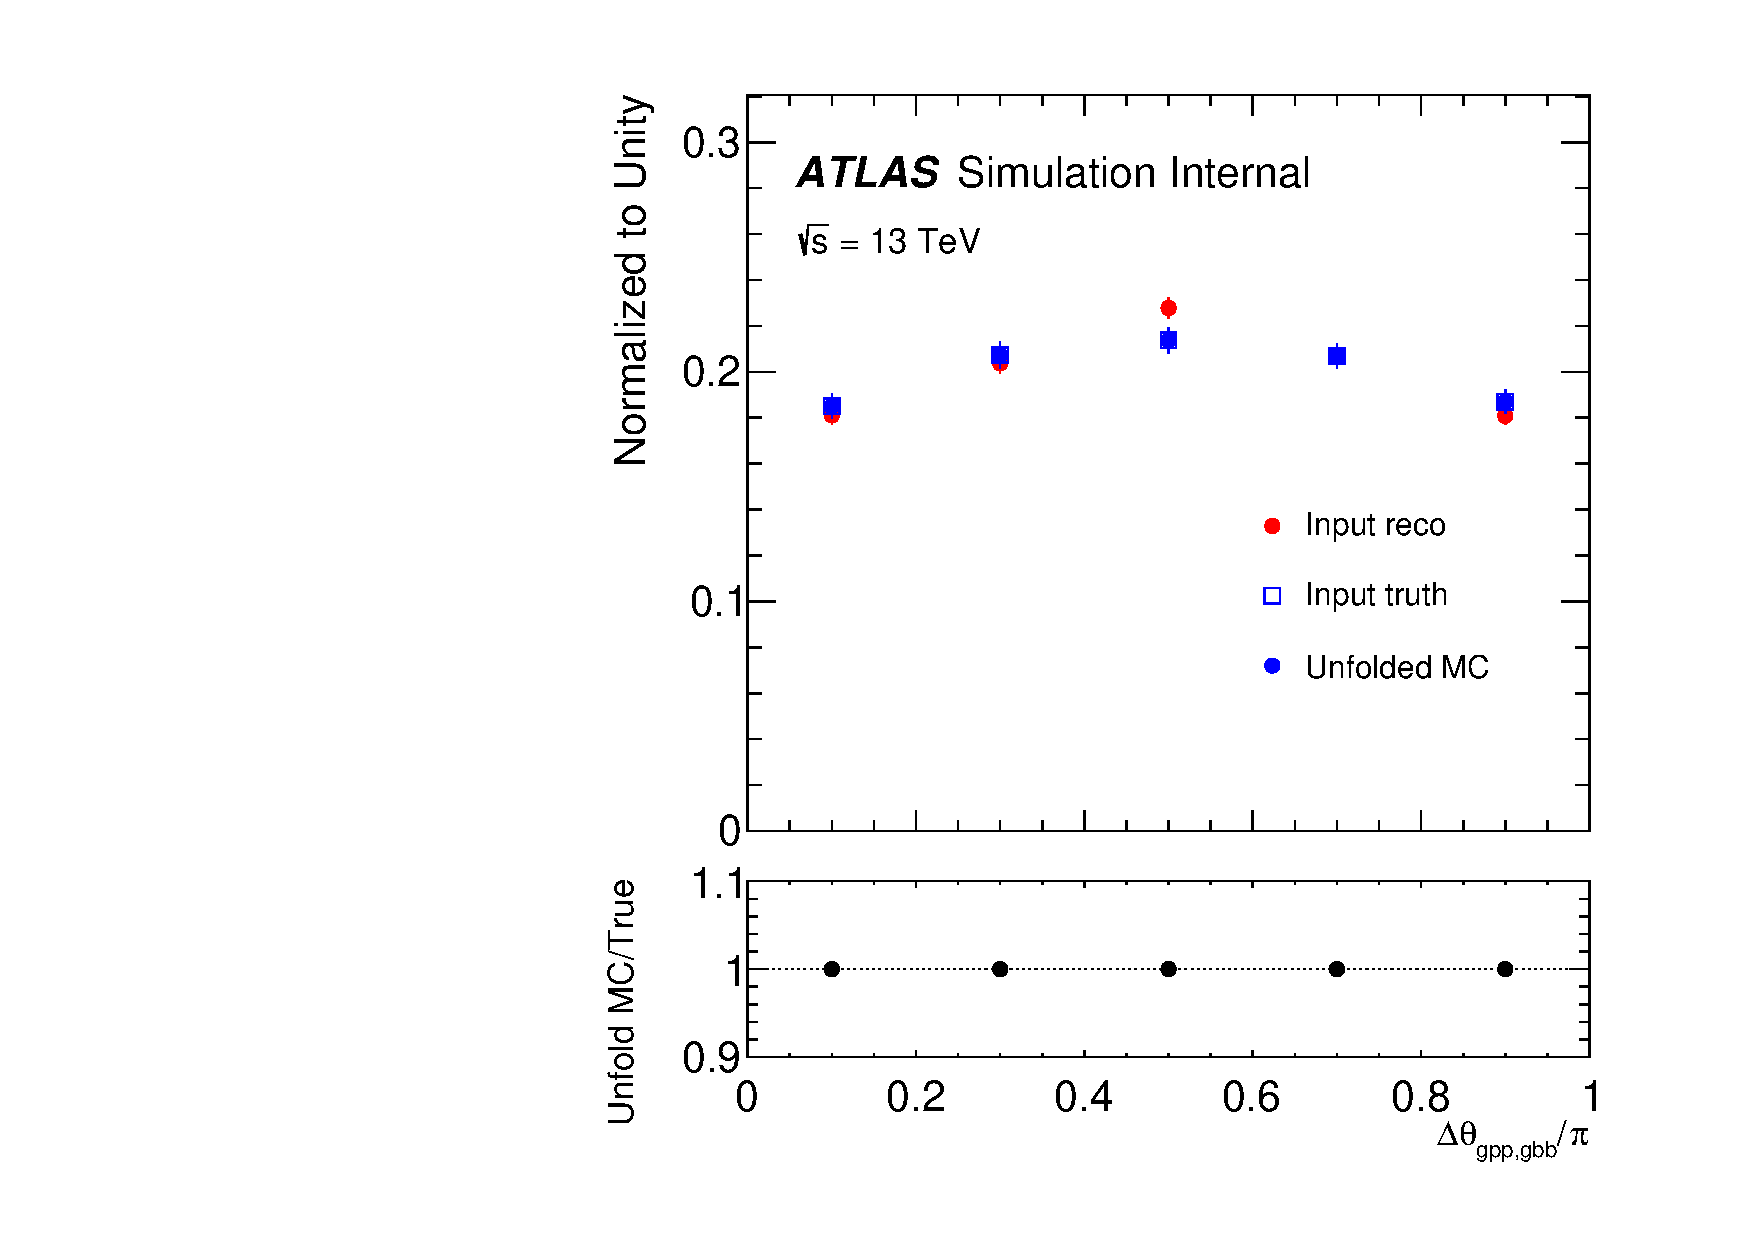
\includegraphics[width=0.45\linewidth]{figures/gbb/Unfolding/dphi_technical_closure.pdf}
  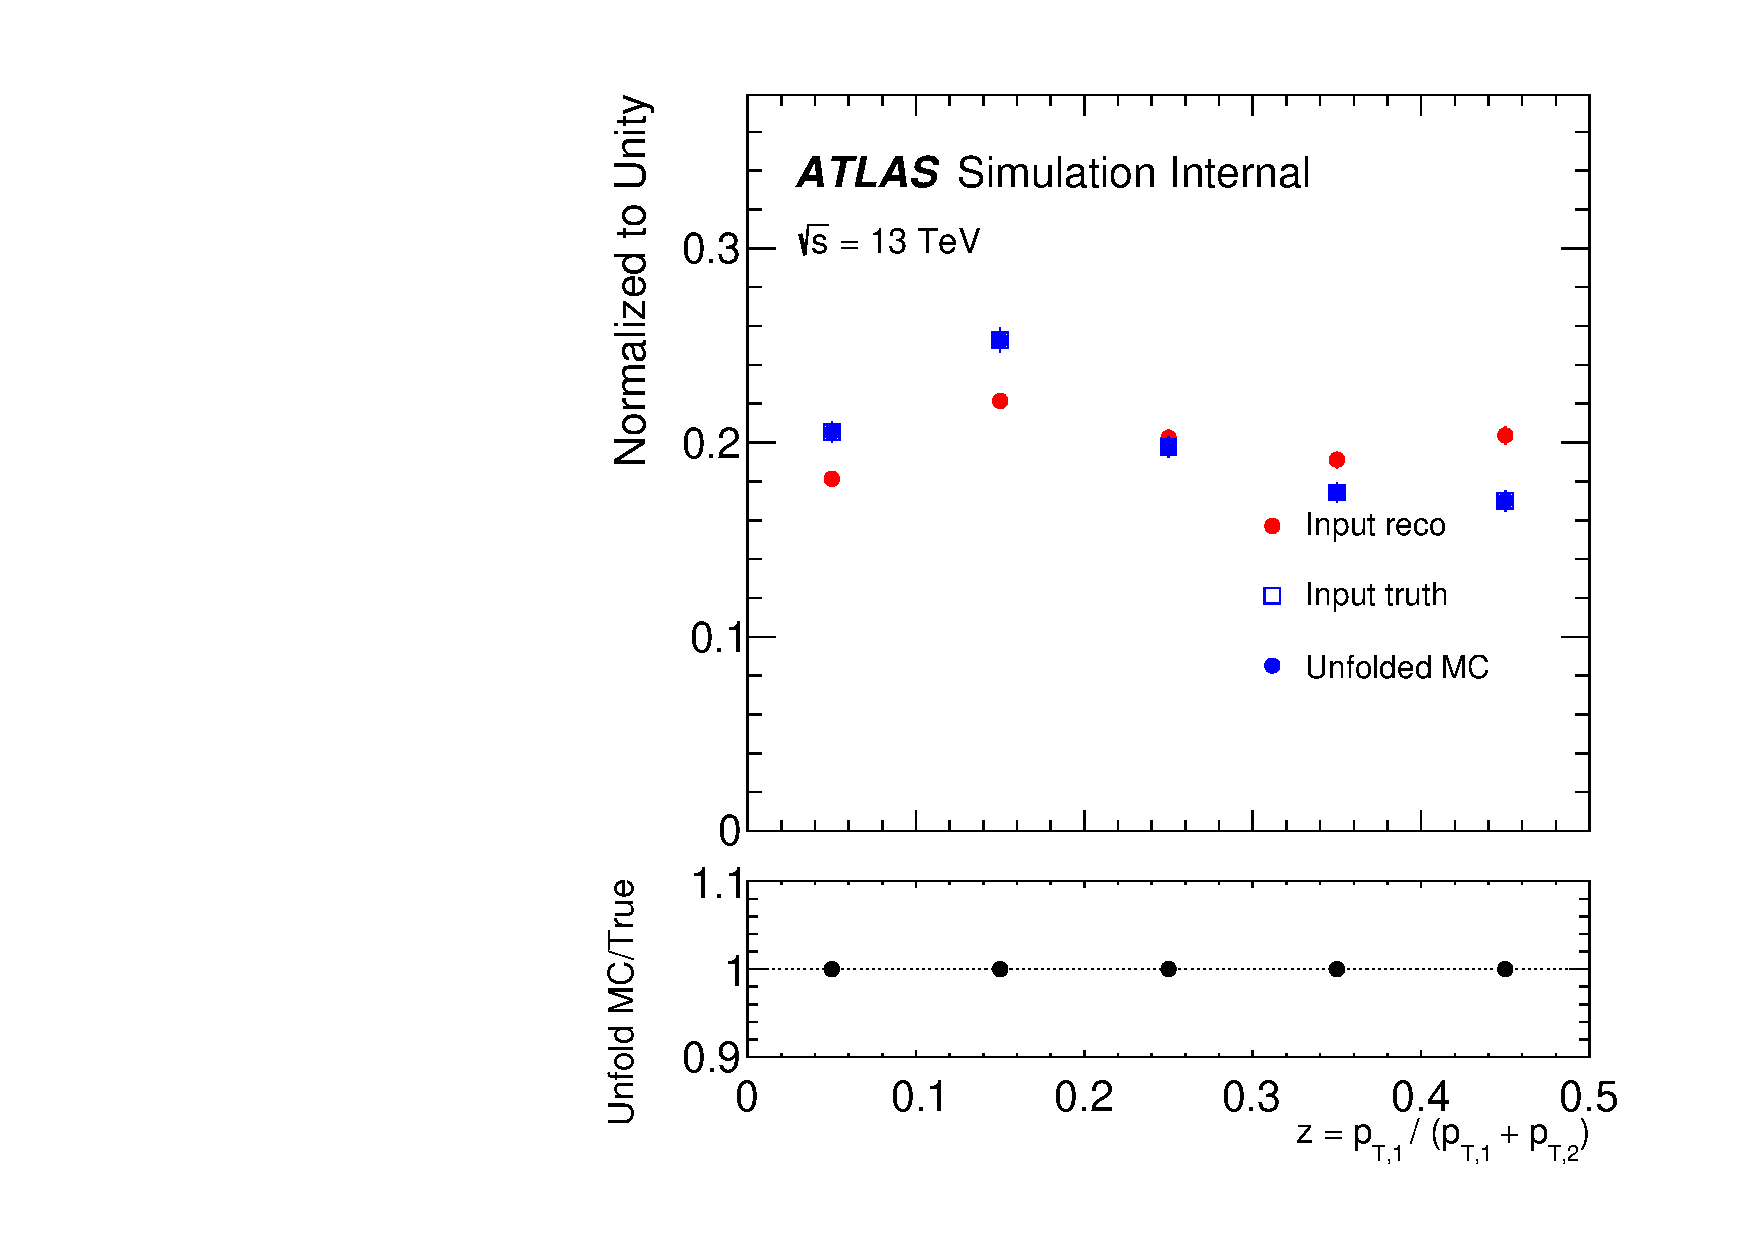
\includegraphics[width=0.45\linewidth]{figures/gbb/Unfolding/ZpT_technical_closure.pdf}
  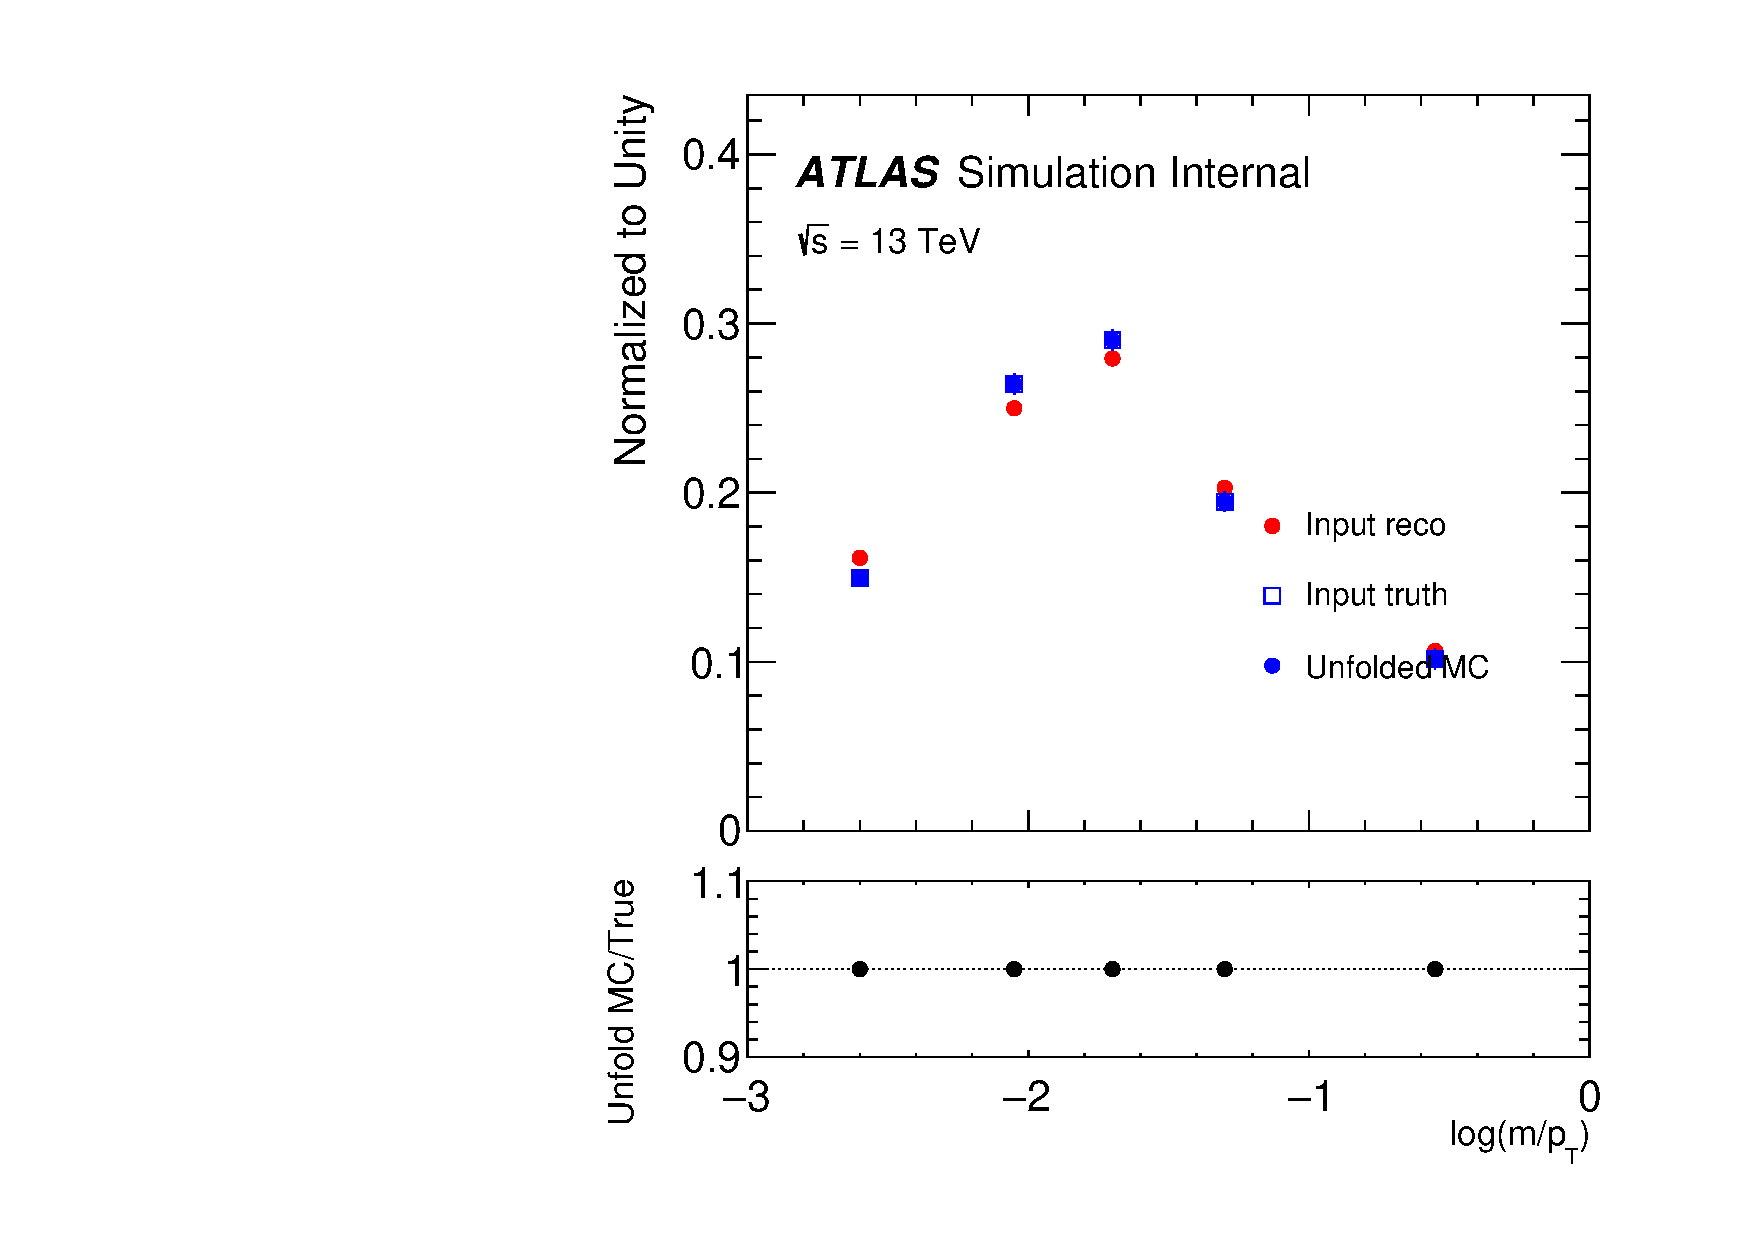
\includegraphics[width=0.45\linewidth]{figures/gbb/Unfolding/fracmasspt_technical_closure.pdf}
\caption[]{A demonstration that the unfolding is not inherently biased.} 
\label{fig:gbb-technicalclosure}
\end{center}
\end{figure}

\subsection{Unfolding Parameter Optimization}
\label{sec:gbb-unfolding:optimization}

We use four iterations and the binning is determined by the background subtraction procedure and not by the diagonality of the response matrix (from that point of view, we could go finer).  Figure~\ref{fig:gbb-iterations} shows the dependence of the uncertainty on the number of iterations.  In some cases, the uncertainty could be smaller by using fewer than four iterations; in all cases, there is nothing to gain from going above four iterations.

 % We could go for finer bins based on the response matrix so that should be okay.  The number of iterations can be checked once all of the uncertainties are in place (though we do not expect a big change from four, which is rather standard for the IB method).


\begin{figure}[htpb!]
\begin{center}
  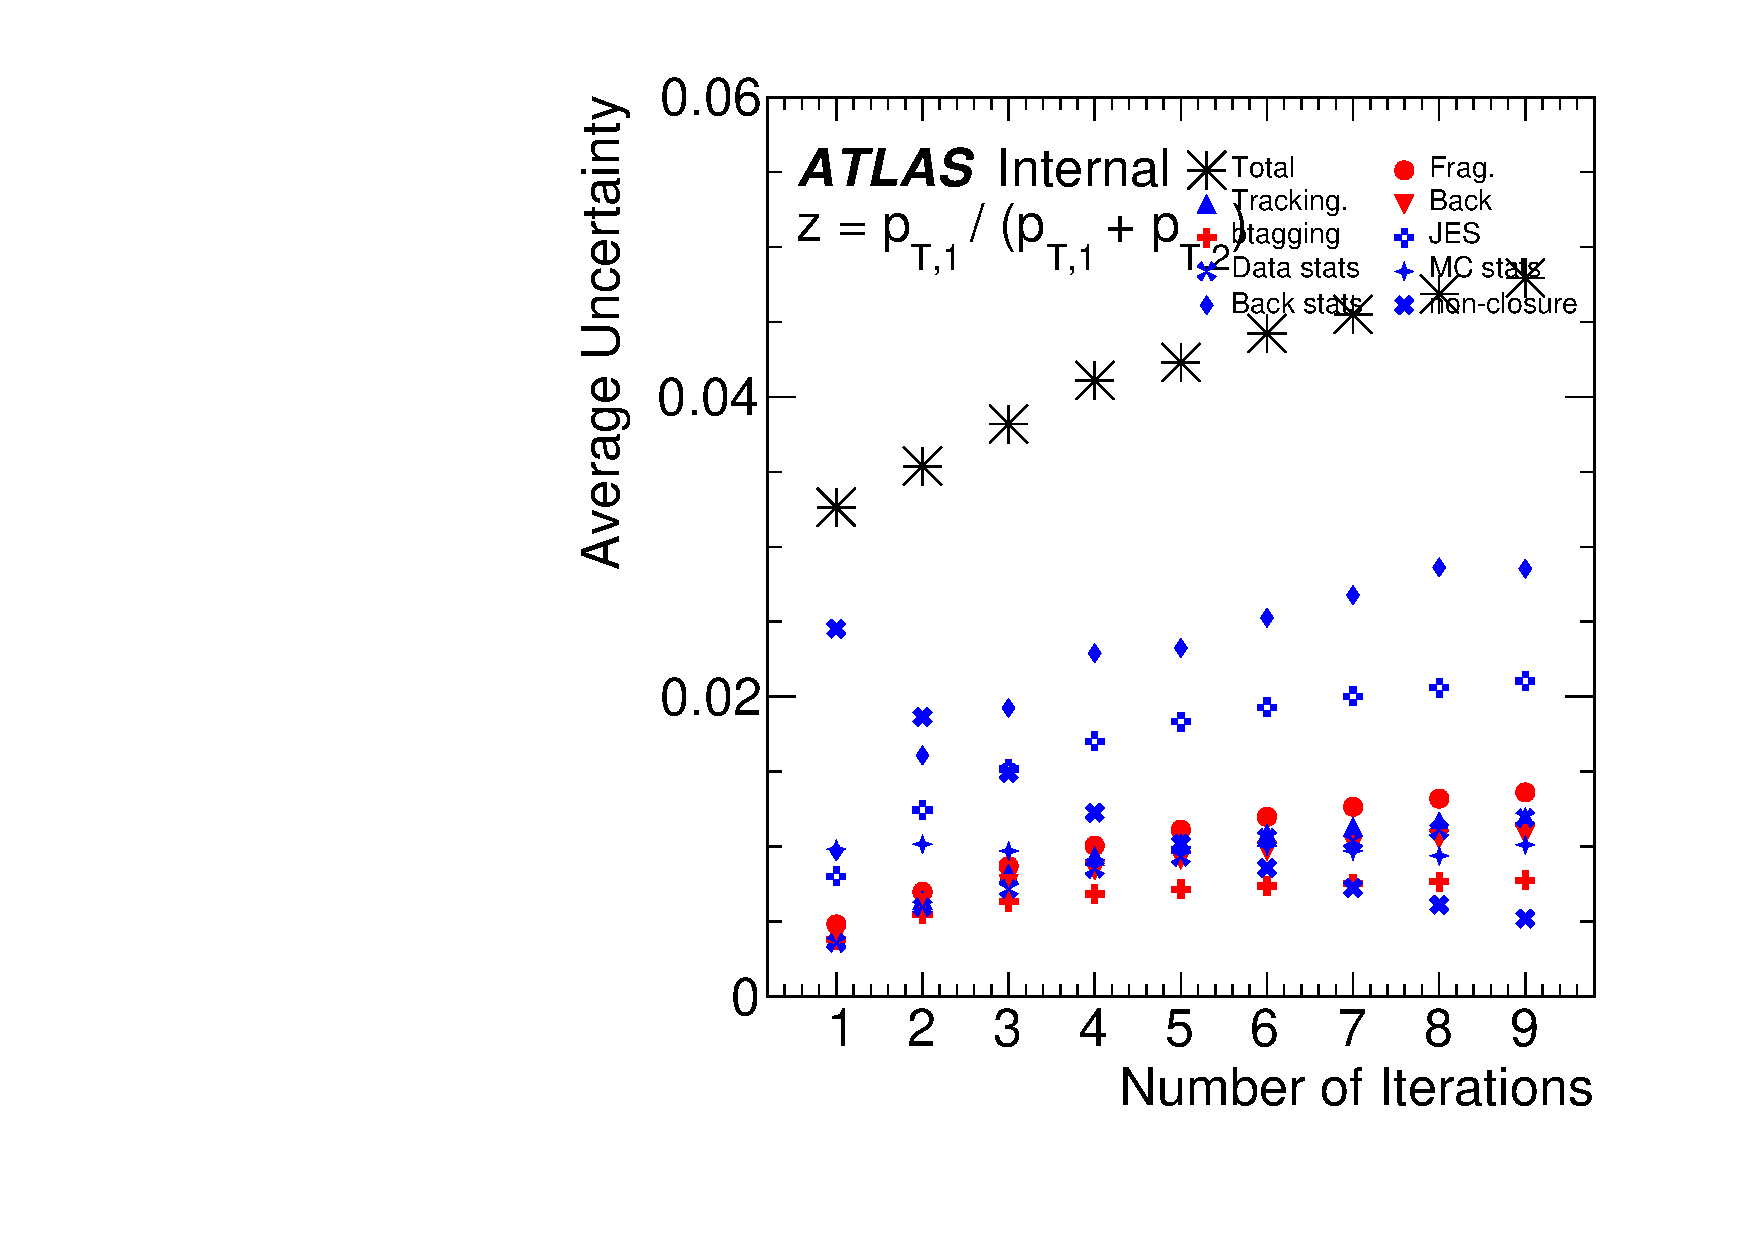
\includegraphics[width=0.45\linewidth]{figures/gbb/Unfolding/IterationsTest_ZpT}
  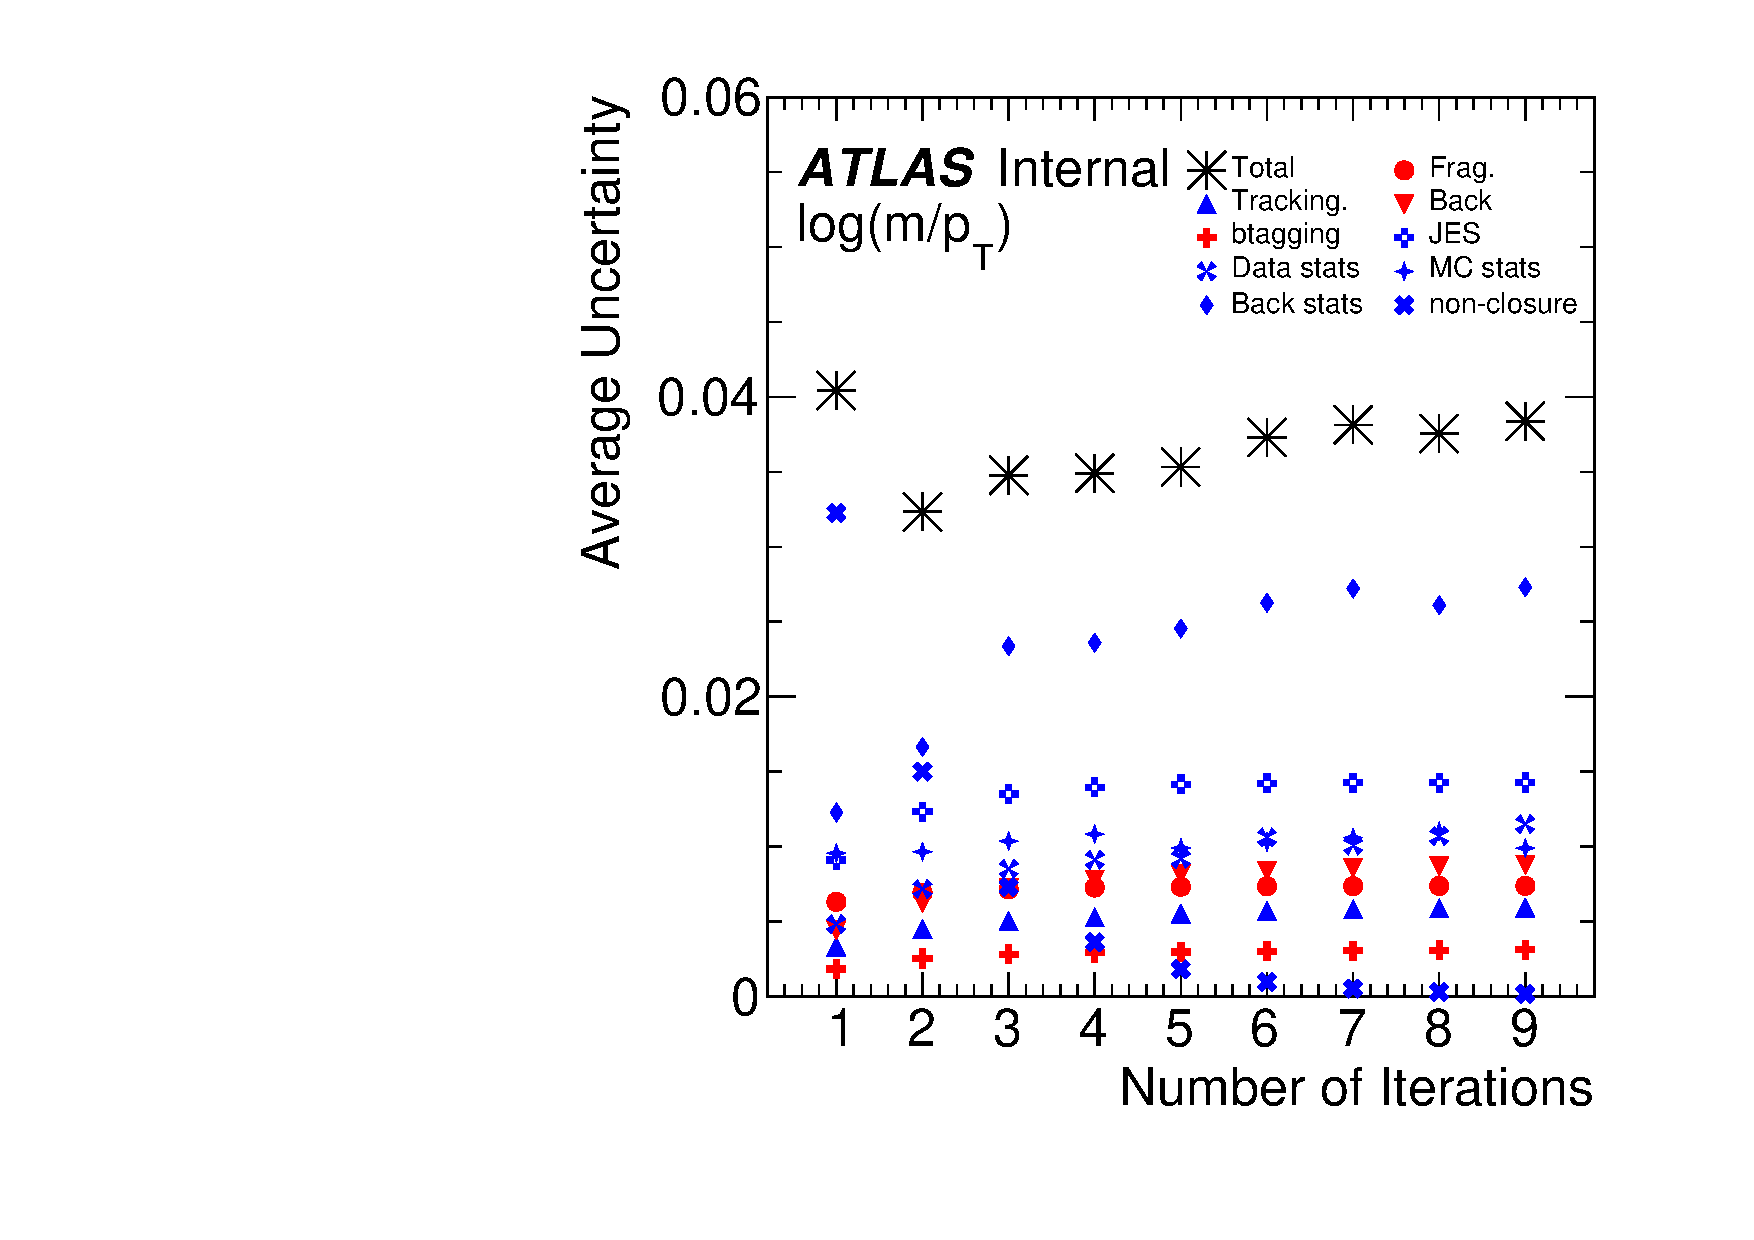
\includegraphics[width=0.45\linewidth]{figures/gbb/Unfolding/IterationsTest_fracmasspt}
  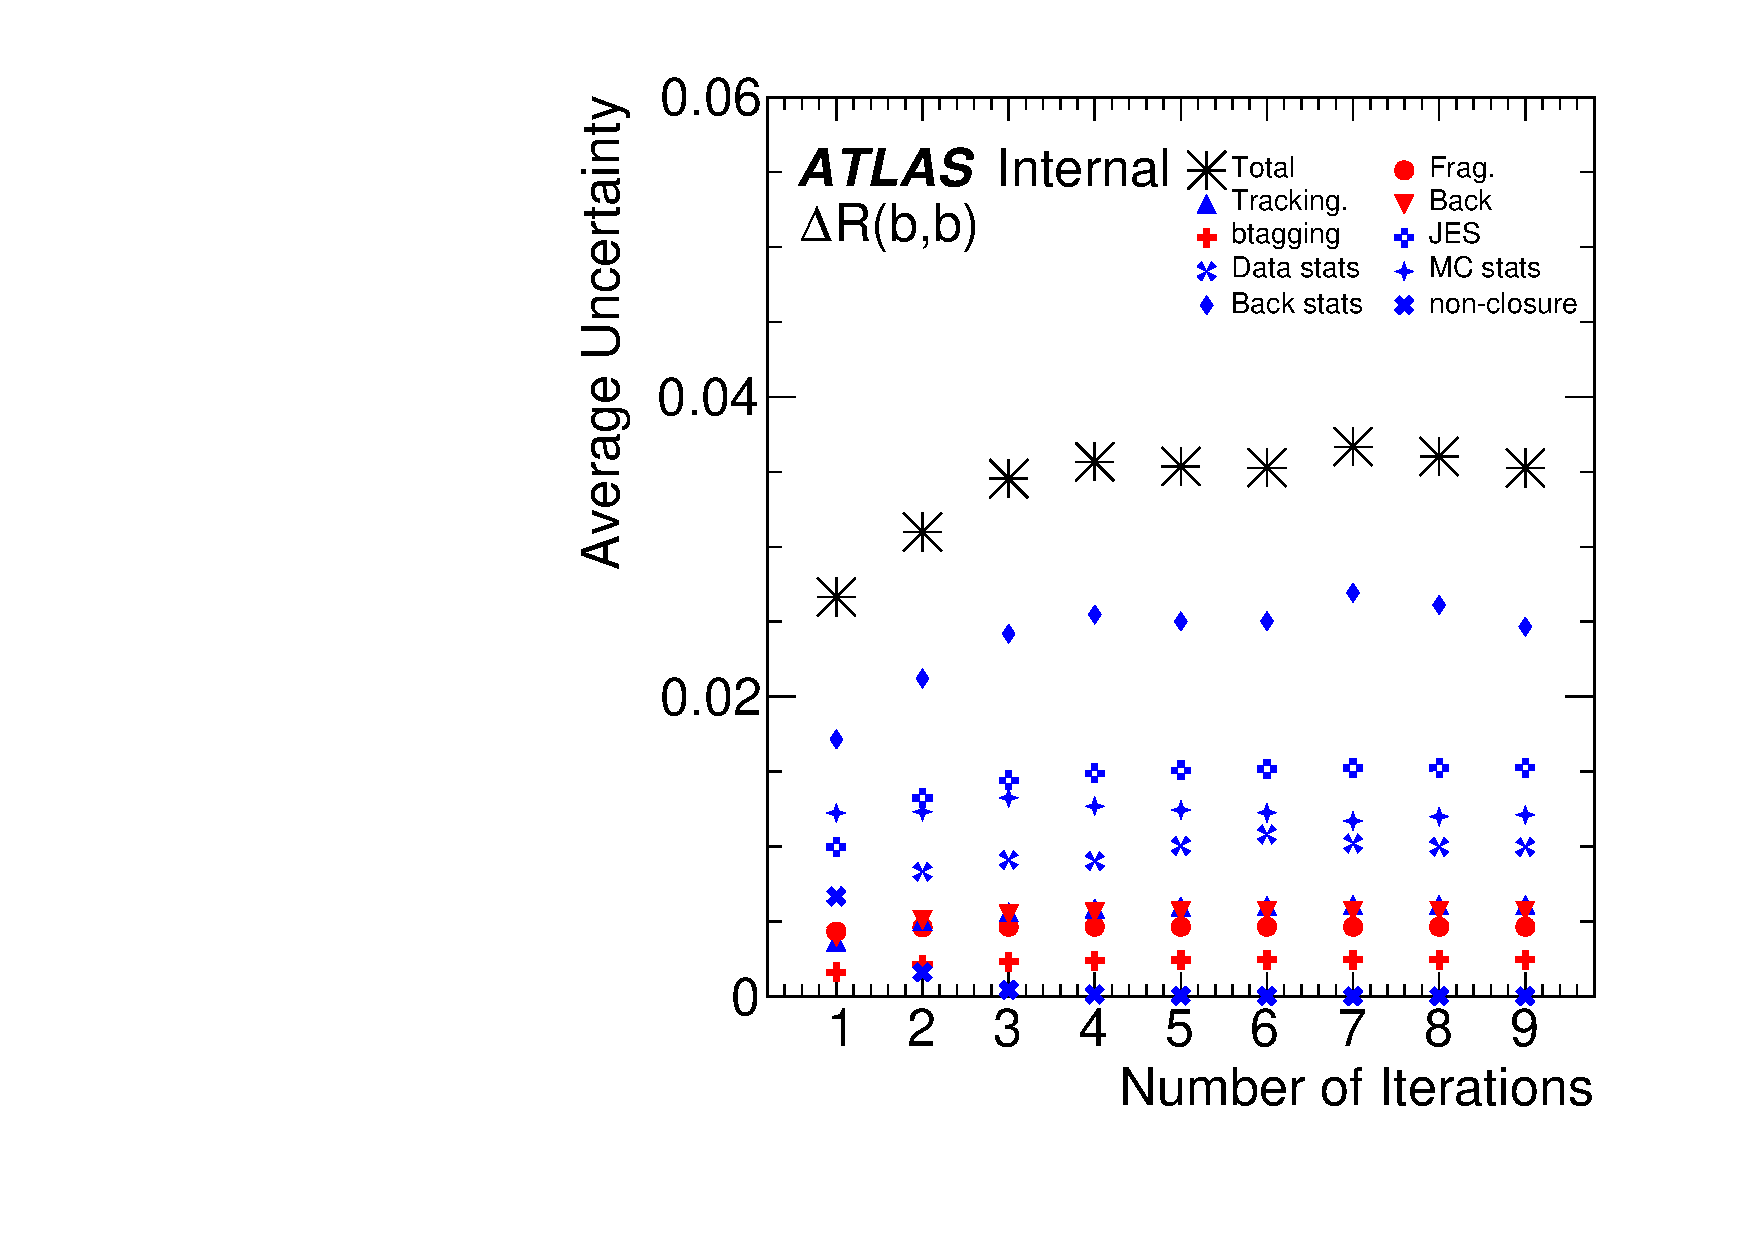
\includegraphics[width=0.45\linewidth]{figures/gbb/Unfolding/IterationsTest_dR}
  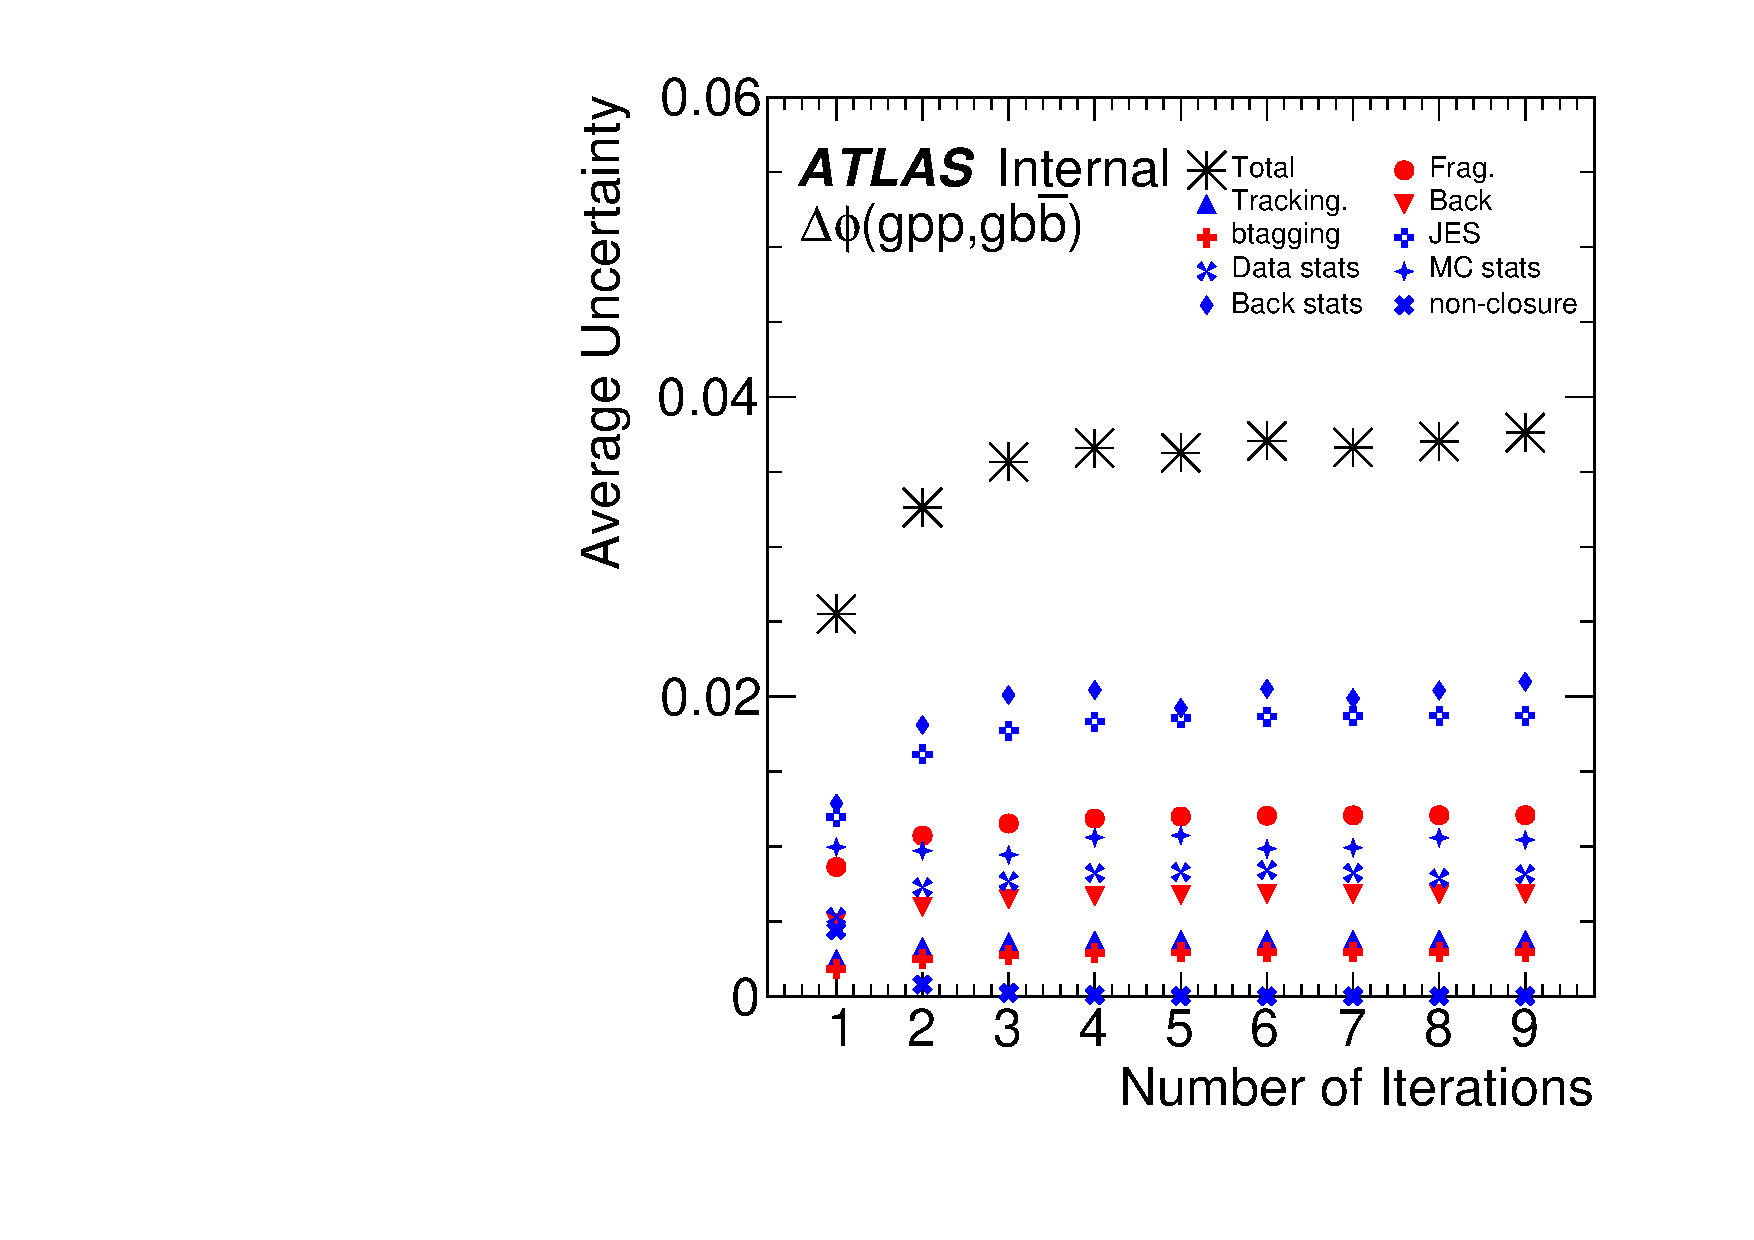
\includegraphics[width=0.45\linewidth]{figures/gbb/Unfolding/IterationsTest_dphi}
\caption[]{The uncertainty as a function of the number of iterations.  See Sec.~\ref{sec:gbb-systs} for a description of the uncertainties. } 
\label{fig:gbb-iterations}
\end{center}
\end{figure}

